\documentclass[acmsmall,screen,anonymous]{acmart}

\usepackage{tabularx}
\usepackage{bbm}
\usepackage{bbold}
\usepackage{mathpartir}
\usepackage{subcaption}
\usepackage{tikz-cd}
\usepackage{xspace}

%\geometry{paperwidth=8.3in, paperheight=11.7in} % force to A4 for now
\settopmatter{printacmref=false}
\citestyle{acmauthoryear}
\raggedbottom

\newcommand*{\note}[1]{\textcolor{blue}{\textbf{note:} #1}}
\newcommand*{\todo}[1]{\textcolor{blue}{\textbf{todo:} #1}}

\newenvironment{salign*}
   {\par\nobreak\small\noindent\csname align*\endcsname}
   {\csname endalign*\endcsname}

\newcommand*{\cat}[1]{\mathbf{#1}}
\newcommand*{\comp}{\circ}
\newcommand*{\eval}{\mathsf{ev}}
\newcommand*{\id}{\mathsf{id}}
\newcommand*{\iso}{\cong}
\newcommand*{\op}{\mathsf{op}}
\newcommand*{\biprod}{\oplus}
\newcommand*{\reindex}[2]{#1[#2]}
\newcommand*{\tensor}{\otimes}
\newcommand*{\zero}{0}

\newcommand*{\One}{\mathbbm{1}}
\newcommand*{\Hom}[3]{{#1}(#2,#3)}

% Specific categories
\newcommand*{\Cat}{\cat{Cat}}
\newcommand*{\CMon}{\cat{CMon}}
\newcommand*{\Fam}{\cat{Fam}}
\newcommand*{\Func}[2]{[#1,#2]}
\newcommand*{\Grothendieck}[1]{\int_{#1}}
\newcommand*{\LatGal}{\cat{LatGal}}
\newcommand*{\Set}{\cat{Set}}
\newcommand*{\Setoid}{\cat{Setoid}}


\begin{document}

\title{Galois Slicing as Differentiation}

\author{Robert Atkey}
\email{robert.atkey@strath.ac.uk}
\orcid{0000-0002-4414-5047}
\affiliation{%
  \institution{University of Strathclyde}
  \city{Glasgow}
  \country{UK}}

\author{Roly Perera}
\email{roly.perera@cl.cam.ac.uk}
\orcid{0000-0001-9249-9862}
\affiliation{%
  \institution{University of Cambridge}
  \city{Cambridge}
  \country{UK}
}
\additionalaffiliation{%
   \institution{University of Bristol}
   \city{Bristol}
   \country{UK}
}

\begin{abstract}
  \GPS is a technique for program slicing for provenance, developed by
  Perera and collaborators. \GPS aims to explain program executions by
  demonstrating how to track approximations of the input and output
  forwards and backwards along a particular execution. In this paper,
  we explore a analogy between \GPS and differentiable programming,
  seeing the implementation of \GPS as a kind of automatic
  differentiation. Using the CHAD approach to automatic differentation
  due to V{\'a}k{\'a} and collaborators, we reformulate \GPS via a
  categorical semantics. In doing so, we are able to explore
  extensions of the \GPS idea to quantitative interval analysis, and
  to clarify the implicit choices made in existing \GPS
  instantiations.
\end{abstract}
\maketitle

\section{Introduction}
\label{sec:introduction}

To audit any computational process, we need robust and well-founded notions of \emph{provenance} to track how data are used. This allows us to answer questions like ``Where did these data come from?'', ``Why are these data in the output?'' and ``How were these data computed?''. Provenance tracking has a wide range of applications, from debugging and program comprehension~\cite{buneman95,cheney07} to improving reproducibility and transparency in scientific workflows~\cite{kontogiannis08}. \emph{Program slicing}, first proposed by~\citet{weiser81}, is a collection of techniques for provenance tracking that attempts to take a run of a program and areas of interest in the output, and turn them into the subset of the input and the program that were responsible for generating those specific outputs.

Existing approaches to program slicing are often tied to particular programming languages or implementations.
In this paper we develop a general categorical approach to program slicing, focusing on a particular technique
called \GPS, where the set of slices of a given value form a lattice of approximations and the forward and
backward slicing procedures generate Galois connections between these lattices. Our main contribution is that
this approach can be seen as a generalised form of automatic differentiation, with slices of values playing
the role of tangents. Our categorical approach should provide a suitable setting for enabling ``automatic''
data provenance for a variety of programming languages, and is easily configured to use alternative
approximation strategies, including quantitative forms of slicing.

\subsection{Galois Program Slicing}
\label{sec:introduction:galois-slicing}

Perera and collaborators introduced the idea of {\em Galois program slicing} as a particular conception of program slicing for provenance, described in several publications~\cite{perera12a,perera16d,ricciotti17}. Galois program slicing (hereafter simply {\emph \GPS}) forms the basis of the open source data visualisation tool \href{https://f.luid.org/}{Fluid}~\cite{perera2025fluid} that allows interactive exploration of programmatically generated visualisations.

At a high level, \GPS assumes that, for each possible value that may be input or output by a program, there exists a lattice of {\em approximations} of that value. For a particular run of a program that takes input $x$ and produces output $y$, we also get a Galois connection between the lattice of approximations of $x$ and the lattice of approximations of $y$. The right half of the Galois connection is the ``forward direction'' taking approximations of the input to approximations of the output; the left half of the Galois connection is the ``backward direction'' that takes approximations of the output to the least (i.e., most approximate) approximation of the input that gives rise to this output approximation. This becomes {\em program slicing} by including the source code of the program as part of the input; then, in the backward direction, the least approximation of the input required for an output approximation includes the least part of the program required as well.

\begin{example}
  \label{ex:introduction-example}
  The following program is written in Haskell syntax \cite{haskell}, using a list comprehension to filter a list of pairs of labels and numbers to those numbers with a given label, and then computing the sum of the numbers:
  \begin{displaymath}
    \begin{array}{l}
      \mathrm{query} :: \mathrm{Label} \to [(\mathrm{Label}, \mathrm{Int})] \to \mathrm{Int} \\
      \mathrm{query}\,l\,\mathit{db} = \mathrm{sum}\,[ n \mid (l',n) \leftarrow \mathit{db}, l \equiv l' ]
    \end{array}
  \end{displaymath}
  With $\mathit{db} = [(\mathsf{a}, 0), (\mathsf{b}, 1), (\mathsf{a}, 1)]$, we will have $\mathit{query}\,\mathsf{a}\,\mathit{db}$ and $\mathit{query}\,\mathsf{b}\,\mathit{db}$ both evaluating to $1$.

  Now suppose that for a given run of the program, we are interested in which of the numerical parts of the input are used to compute the output for the query parameters $l = \mathsf{a}$ and $l = \mathsf{b}$. We can use \GPS to do this. We arrange for the approximations of the input to form the following lattice, where the actual piece of data is at the top and information lost by approximation is represented by $\bot$s:
  \begin{center}
    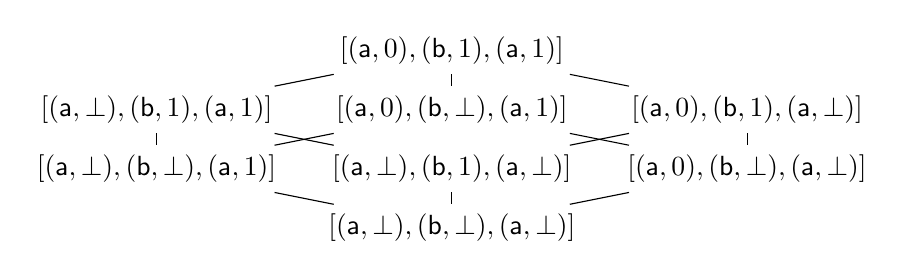
\begin{tikzpicture}[node distance=0.75cm]
      \node (top) at (0,0) {$[(\mathsf{a}, 0), (\mathsf{b}, 1), (\mathsf{a}, 1)]$};
      % row 2
      \node [below of=top] (ioi) {$[(\mathsf{a}, 0), (\mathsf{b}, \bot), (\mathsf{a}, 1)]$};
      \node [left of=ioi,xshift=-3cm] (oii) {$[(\mathsf{a}, \bot), (\mathsf{b}, 1), (\mathsf{a}, 1)]$};
      \node [right of=ioi,xshift=3cm] (iio) {$[(\mathsf{a}, 0), (\mathsf{b}, 1), (\mathsf{a}, \bot)]$};
      % row 3
      \node [below of=ioi] (oio) {$[(\mathsf{a}, \bot), (\mathsf{b}, 1), (\mathsf{a}, \bot)]$};
      \node [left of=oio,xshift=-3cm] (ooi) {$[(\mathsf{a}, \bot), (\mathsf{b}, \bot), (\mathsf{a}, 1)]$};
      \node [right of=oio,xshift=3cm] (ioo) {$[(\mathsf{a}, 0), (\mathsf{b}, \bot), (\mathsf{a}, \bot)]$};
      % row 4
      \node [below of=oio] (bot) {$[(\mathsf{a}, \bot), (\mathsf{b}, \bot), (\mathsf{a}, \bot)]$};

      % links
      \draw (top) -- (ioi);
      \draw (top) -- (oii);
      \draw (top) -- (iio);
      \draw (ioi) -- (ooi);
      \draw (ioi) -- (ioo);
      \draw (oii) -- (ooi);
      \draw (oii) -- (oio);
      \draw (iio) -- (ioo);
      \draw (iio) -- (oio);
      \draw (ooi) -- (bot);
      \draw (oio) -- (bot);
      \draw (ioo) -- (bot);
    \end{tikzpicture}
  \end{center}
  In both runs of the program, the output approximation lattice looks like this, where $1$ is the actual data point that was returned, and $\bot$ indicates that we are approximating this piece of data away:
  \begin{center}
    \begin{tikzpicture}[node distance=0.75cm]
      \node (top) at (0,0) {$1$};
      \node [below of=top] (bot) {$\bot$};
      \draw (top) -- (bot);
    \end{tikzpicture}
  \end{center}
  These are not the only choices of approximation lattices that we could have made. For the input, we have chosen a lattice that allows us to ``forget'' (approximate away) numbers in the input, but not the labels or the structure of the list itself. However, other choices are also useful. Indeed, one of the aims of this work is to clarify how to choose an approximation structure appropriate for different tasks by use of type information. We elaborate on this further in \secref{semantic-gps}.

  \GPS associates with each run of the program a Galois connection telling us how the inputs and outputs are related in that run. The backwards portion $\partial (\mathit{query}\,l)_r$ tells us, given an approximation of the output, what the least approximation of the input is needed to generate that output. In the case of the two runs considered in this example, if we say we are not interested in the output by feeding in the least approximation $\bot$, then we find that we only need the least approximation of the input:
  \begin{displaymath}
    \partial (\mathit{query}\,l\,\mathit{db})_r(\bot) = [(\mathsf{a},\bot), (\mathsf{b}, \bot), (\mathsf{a}, \bot)]
  \end{displaymath}
  for both $l = \mathsf{a}$ and $l = \mathsf{b}$. If instead we take the greatest approximation of the output (i.e., the output ``$1$'' itself), then the two query runs' backwards approximations return different results:
  \begin{displaymath}
    \begin{array}{l}
      \partial (\mathit{query}\,\mathsf{a}\,\mathit{db})_r(1) = [(\mathsf{a},0), (\mathsf{b},\bot), (\mathsf{a},1)] \\
      \partial (\mathit{query}\,\mathsf{b}\,\mathit{db})_r(1) = [(\mathsf{a},\bot), (\mathsf{b},1), (\mathsf{a},\bot)]
    \end{array}
  \end{displaymath}
  Pieces of the input that were {\em not} used are replaced by $\bot$. As we expect, the run of the query with label $\mathsf{a}$ depends on the entries in the database labelled with $\mathsf{a}$, and likewise for the run with label $\mathsf{b}$.

  In this case, the forwards portion of the Galois connection tells us, for each approximation of the input, whether or not it is sufficient to compute the output. If we provide insufficient data to compute the output, then we will get an underapproximated output. Here for example we will find that $\partial (\mathit{query}\, \mathsf{a})_f([(\mathsf{a},0),(\mathsf{b},\bot),(\mathsf{a},\bot)]) = \bot$ because we need all the values associated with the label $\mathsf{a}$ to compute their sum.

  In a simple query like this, it is easy to work out the dependency relationship between the input and output. However, the benefit of \GPS, and other language-based approaches, is that it is {\em automatic} for all programs, no matter how complex the relationship between input and output. Moreover, by changing what we mean by ``approximation'' we can compute a range of different information about a program.
\end{example}

\subsection{Galois Slicing and Automatic Differentiation}

Previous work on \GPS used a special operational semantics to generate a trace of each execution, and then uses that trace to compute the Galois connections described above, by re-running forwards or backwards over the trace. It would be useful to have a denotational account of \GPS as well, especially if we could provide a semantics where the backwards analysis is baked in, rather than provided by a separately defined ``backwards evaluation'' operation. Our thesis, developed in \secref{approx-as-tangents} and \secref{models-of-total-gps} is that there is a close analogy between \GPS and \emph{automatic differentiation} for differentiable programs~\cite{siskind08,elliott18,vakar22}, which points to a way to develop such an approach. We have already hinted at this in the description above, but let us now make it explicit.

\begin{itemize}[leftmargin=\enummargin]
\item For \GPS, we assume that every value has an associated lattice of {\em approximations}. For differentiable programs, every point has an associated vector space of {\em tangents}.
\item For \GPS, every program has an associated forward approximation map that takes approximations forward from the input to the output. This map {\em preserves meets}. For differentiable programs, every program has a forward derivative that takes tangents of the input to tangents of the output. The forward derivative map is {\em linear}, so it preserves addition of tangents and the zero tangent.
\item For \GPS, every program has an associated backward approximation map that takes approximations of the output back to least approximations of the input. This map {\em preserves joins}. For differentiable programs, every program has a reverse derivative that takes tangents of the output to tangents of the input. This map is again {\em linear}.
\item For \GPS, the forward and backward approximation maps are related by being a Galois connection. For differentiable programming, the forward and reverse derivatives are related by being each others' transpose.
\end{itemize}

Given this close connection between \GPS and differentiable programming, we can take structures intended for modelling automatic differentiation, such as V{\'a}k{\'a}r's CHAD framework and use them to model \GPS. This will enable us to generalise and expand the scope of \GPS to act as a foundation for data provenance in a wider range of computational settings.

\subsection{Outline and Contributions}

%Our primary contribution in this article is to elucidate \GPS by relating it to differentiable programming and automatic differentiation. In doing so, we aim to expand the applicability of program slicing, and to potentially transfer efficient automatic differentiation implementation techniques from automatic differentiation to program slicing and provenance tracking.

\GPS, as any program slicing technique, essentially rests on an analysis of how programs intensionally explore their input, in addition to their extensional behaviour. Such analysis has been carried out over many years in Domain Theory. In \secref{approx-as-tangents}, we use ideas from \citet{berry79}'s \emph{stable domain theory} and develop an analogy between stable functions and smooth functions from mathematical analysis, where stable functions provide a kind of semantic provenance analysis. In \secref{models-of-total-gps}, we abstract from stable functions using V{\'a}k{\'a}r \etal{}'s CHAD framework \cite{vakar22,nunes2023} to build models of a higher-order language that automatically compute slices. We apply this to a concrete higher-order language in \secref{language} and demonstrate the use of the model on variations of \exref{introduction-example}, highlighting the flexibility of our approach. In particular, we show how type structure can be used to control the approximation lattices associated with data points, something that was ``hard coded'' in previous presentations of \GPS. We prove two correctness properties in \secref{definability}, relating the higher-order interpretations to first-order ones, proving the crucial Galois connection property. \secref{related-work} and \secref{conclusion} discuss additional related and future work.

% \begin{enumerate}[leftmargin=\enummargin]
% \item We explain how the CHAD framework of Vákár et al. can be adapted to give a general categorical framework for \GPS.
% \item Using our adapted CHAD framework, we can explain how type structure can be used to control the approximation lattices associated with data points, something that was ``hard coded'' in previous presentations of \GPS.
% \item With the benefit of our abstract setting, we can relate \GPS to other parts of denotational semantics. In particular, we show that there is a close connection with Stable Domain Theory, a proposed solution to capturing sequentiality by recording more intensional information about programs' sensitivity to approximations.
% \end{enumerate}

We have formalised our major results in Agda, resulting in an executable implementation built directly from the categorical constructions that we have used to compute the examples in \secref{language:examples}. Please consult the file \texttt{everything.agda} in the supplementary material.


% \begin{enumerate}
% \item We explain how the CHAD framework of Vákár et al. can be adapted to give a general categorical framework for \GPS.
% \item Using our adapted CHAD framework, we can explain how type structure can be used to control the approximation lattices associated with data points, something that was ``hard coded'' in previous presentations of \GPS.
% \item With the benefit of our abstract setting, we can relate \GPS to other parts of denotational semantics. In particular, we show that there is a close connection with Stable Domain Theory, a proposed solution to capturing sequentiality by recording more intensional information about programs' sensitivity to approximations.

% We have \anonymise{\href{https://github.com/bobatkey/approx-diff}{formalised this work in Agda}}{formalised this work in Agda}. Not only does this mean that the constructions and proofs have been checked, but also the construction is executable and can be run on small examples. We are also planning to use Agda's JavaScript backend to produce a demo.

\section{Approximations as Tangents}
\label{sec:approx-as-tangents}

We motivate our approach to \GPS by showing how to combine ideas from differential geometry and stable domain theory to reconstruct \GPS in a denotational setting. From this basis, we apply the CHAD framework of V{\'a}k{\'a}r \etal to obtain a denotational model of automatic differentiation that gives us an effective way to interpret programs as functions along with their forward and backwards approximation maps\bob{and we did it in Agda, so we can run it}.

\subsection{Manifolds, Smooth Functions, and Automatic Differentiation}

% For what follows we do not need to know in detail what a manifold is, or exactly how smooth functions are defined. We only state some definitions in order to fix terminology and to justify our claim of a connection to manifolds and smooth functions. \bob{Need a good reference here.}

The general study of differentiable functions takes place on \emph{manifolds}, which are topological spaces that ``locally'' look like a subset of the Euclidean space $\RR^n$. The spaces $\RR^n$ themselves are manifolds, but so are ``non-flat'' examples such as $n$-spheres and yet more exotic spaces. Every point $x$ in a manifold $M$ has an associated \emph{tangent vector space} $\tangents_x(M)$ and \emph{cotangent vector space} $\cotangents_x(M)$, the latter consisting of linear functions $\tangents_x(M) \linearto \RR$. The tangent and cotangent spaces are finite dimensional, so in the presence of a chosen basis they are canonically isomorphic. In the case when the manifold is $\RR^n$, then every tangent space is isomorphic to $\RR^n$ as well.

Smooth functions $f$ between manifolds $M$ and $N$ are functions on their points that are locally differentiable on $\RR^n$. Each smooth function induces maps of the (co)tangent spaces:
\begin{itemize}
\item The \emph{forward derivative} (tangent map or pushforward) $\pushf{f}_x$ is a linear map $\tangents_x(M) \linearto \tangents_{f(x)}(N)$. In the Euclidean case when $M = \RR^m$ and $N = \RR^n$, the tangent map can be represented by the Jacobian matrix of partial derivatives of $f$ at $x$.
\item The \emph{backward derivative} (cotangent map, or pullback) $\pullf{f}_x$ is a linear map $\cotangents_{f(x)}(N) \linearto \cotangents_x(M)$. In the Euclidean case, the backward derivative is represented by the transpose of the Jacobian of $f$ at $x$.
\end{itemize}

Computing the forward and backward derivatives of smooth functions $f$ has many applications of practical interest. For example, computation of the reverse derivative is of central interest in Machine Learning by Gradient Descent, the main technique used to train Deep Neural Networks. \bob{need a citation here}.

Derivatives can be computed numerically by computing $f$ on small perturbations of its input, or symbolically by examining a closed-form representation of $f$. However, a more common and practical technique is to use \emph{automatic differentiation}, where a program computing $f$ is instrumented to produce (a representation of) the forward and/or backward derivative as a side-effect of producing the output. \bob{cite something on autodiff}. This has led to the area of differentiable programming, where programming languages and their implementations are specifically designed to admit efficient automatic differentation algorithms. \bob{cite: JAX, TensorFlow, Dex, Jesse Sigal, etc.}

\subsection{Stable Domain Theory as Differentiability}

Our thesis is that \GPS is a form of differentiable programming, where tangents are not linear approximations of functions but instead are qualitiative approximations of elements in the sense of domain theory. Smooth functions in this setting are Berry's \emph{stable functions} \cite{berry79,berry82}. We now introduce these concepts and how they relate to \GPS.

\subsubsection{Domains as a Qualitative Theory of Approximation}

Domain theory is a method for defining the semantics of programs that handle infinite data (e.g., functions or infinite streams). \emph{Domains} are certain partially ordered sets where the ordering denotes a relationship of qualitative information content: if $x \sqsubseteq y$, then $y$ may contain more information than $x$. For example, if $x$ and $y$ are functions, then $y$ may be defined for more values in its domain than $x$. Infinite objects are understood in terms of their approximations in this sense, and domains are assumed to be closed under least upper bounds (lubs) of directed sets, meaning that any internally consistent collection of elements has a ``completion'' that contains all the information covered by the set. Programs are interpreted as monotone functions that preserve directed lubs. Monotonicity captures the idea that if the input gets more defined, then the output can get more defined. Preservation of lubs, or \emph{continuity}, states that a function interpreting a program cannot act inconsistently on approximations and their completion, which corresponds to the intuitive idea that a function that is computable cannot look at a non-finite amount of input to produce a finite output.

For the purposes of \GPS, we are not interested in using approximations to model computation on infinite objects, but instead to use them for the related use of revealing how programs explore their inputs when producing parts of their output. Therefore, we ignore completeness properties of the partially ordered sets we consider.

\subsubsection{Stable Functions as ``Smooth Functions''}

%FIXME: use cleverref

When giving a denotational semantics for sequential programming languages, such as PCF, continuous functions are too permissive. Plotkin's Parallel OR (\autoref{ex:parallel-or}, below) is continuous but does not treat its input in a way that is consistent with a sequential implementation \cite{plotkin77lcf}. Continuous functions can explore their input in a ``random access'' way, which is incompatible with the central idea in \GPS that we should be able to identify a \emph{minimal} part of the input that leads to a part of the output.

Stability is a property that can be required of monotone functions that was invented by Berry~\cite{berry79} in an attempt to capture sequentiality. This was not successful (see the $\mathrm{gustave}$ function in \autoref{ex:parallel-or}), but we will see now how it is closely related to problem of computing forward and backwards maps of approximations needed in \GPS. A textbook description of stable functions in the context of domain theory is given by \citet{amadio-curien} (Chapter 12). We start with a property that is weaker than stability, but is easier to motivate in connection with derivatives of smooth functions.

In a partially ordered set $X$, for any $x \in X$ the set of elements below $x$, $\downset{x} = \{ x' \mid x' \sqsubseteq x \}$, is itself a partially ordered set. These approximations of $x$ we will think of as ``derivatives'' of $x$, and the whole set $\downset{x}$ as the ``tangent space''. Tangent spaces are vector spaces, since they are linear approximations to curves at that point. In the partially ordered setting, we take elements of $\downset{x}$ to be approximations of processes defined at $x$. As we can add tangents, we assume we can take meets of approximations in $\downset{x}$:

\begin{definition}
  A \emph{bounded meet poset} is a partially ordered set $X$ where for every $x \in X$, $\downset{x}$ is a meet semilattice, with $x$ as the top element.
\end{definition}

Smooth functions have a ``pushforward'' derivative that takes tangents at a point $x$ to tangents at the point $f(x)$ and is linear. In the partially ordered setting, we are going to take a function $f$'s pushforward derivative at $x$ to be its restriction to $\downset{x}$, taking approximations of the input to approximations of the output. Matching the linearity of the pushforward derivative smooth functions, we require that these restrictions preserve meets:

\begin{definition}
  A \emph{conditionally multiplicative} (cm) function $f : X \to Y$ is
  a monotone function such that for all $x \in X$, the restriction
  $f_x : \downset{x} \to \downset{f(x)}$ preserves meets.
\end{definition}

\begin{lemma}
  Morphisms of meet approximation spaces are closed under identities
  and composition, forming a category. FIXME: with products?
  functions? sums?
\end{lemma}

\begin{example}[Conditionally Multiplicative Functions]
\label{ex:strict-short-circuit}
  To see the effect of requiring preservation of bounded meets,
  consider several ways of defining disjunction on the lifted booleans
  $\mathbb{B}_\bot$. Two functions that are cm are the strict and
  left-short-circuiting ORs\footnote{The clauses in these examples are
    shorthand for the graph of the function. They are not to be
    understood as pattern matching clauses in a language like Haskell,
    where it is not possible to match on $\bot$.}:
  \begin{displaymath}
    \begin{array}[t]{l@{(}l@{,~}l@{)~}c@{~}l}
      \mathrm{strictOr}&\mathsf{tt}&\mathsf{tt}&=&\mathsf{tt} \\
      \mathrm{strictOr}&\mathsf{tt}&\mathsf{ff}&=&\mathsf{tt} \\
      \mathrm{strictOr}&\mathsf{ff}&\mathsf{tt}&=&\mathsf{tt} \\
      \mathrm{strictOr}&\mathsf{ff}&\mathsf{ff}&=&\mathsf{ff} \\
      \mathrm{strictOr}&\bot&\_&=&\bot \\
      \mathrm{strictOr}&\_&\bot&=&\bot \\
    \end{array}
    \qquad
    \begin{array}[t]{l@{(}l@{,~}l@{)~}c@{~}l}
      \mathrm{shortCircuitOR}&\mathsf{tt}&\_&=&\mathsf{tt} \\
      \mathsf{shortCircuitOR}&\mathsf{ff}&x&=&x \\
      \mathsf{shortCircuitOR}&\bot&\_& =& \bot
    \end{array}
    \qquad
    \raisebox{-15ex}{
      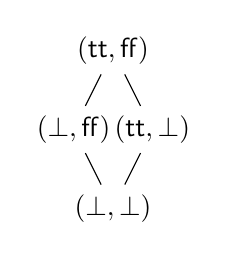
\begin{tikzpicture}
        \node (top) at (0,0) {$(\mathsf{tt},\mathsf{ff})$};
        \node [below of=top,xshift=-0.5cm] (oi) {$(\bot,\mathsf{ff})$};
        \node [below of=top,xshift=0.5cm] (io) {$(\mathsf{tt},\bot)$};
        \node [below of=oi,xshift=0.5cm] (oo) {$(\bot,\bot)$};
        \draw (top) -- (oi);
        \draw (top) -- (io);
        \draw (oi) -- (oo);
        \draw (io) -- (oo);
      \end{tikzpicture}
    }
  \end{displaymath}
  In the poset $\mathbb{B}_\bot^2$, a typical poset of approximations of a fully defined element is shown to the right. For $\mathrm{strictOr}$, any approximation that isn't the fully defined input is mapped to $\bot$, while $\mathrm{shortCircuitOr}$ maps the partially defined $(\mathsf{tt},\bot)$ to $\mathsf{tt}$. Thus, even though these functions operate identically on fully defined inputs, they differ in their \emph{derivatives} on partially defined input, exposing how . That they are cm can be checked by examining their restrictions' behaviour. If we take the approximations $(\bot,\mathsf{ff})$ and $(\mathsf{tt},\bot)$, then their meet is $(\bot,\bot)$; $\mathrm{strictOr}$ maps all three elements to $\bot$, so is cm here since $\bot \wedge \bot = \bot$; and $\mathrm{shortCircuitOR}$ has $(\bot,\mathsf{ff}) \mapsto \bot$ and $(\mathsf{tt},\bot) \mapsto \mathsf{tt}$, the meet of which is $\bot = \mathrm{shortCircuitOR}(\bot,\bot)$. Other combinations can be checked similarly.
\end{example}

\begin{example}[A non-Conditionally Multiplicative Function]
  \label{ex:parallel-or}
  A function that is not cm is Plotkin's Parallel OR \cite{lcf77}, which short-circuits in both arguments. It returns $\mathsf{tt}$ if either argment is $\mathsf{tt}$ even if the other argument is not defined:
  \begin{displaymath}
    \begin{array}{l@{(}l@{,~}l@{)~}c@{~}l}
      \mathrm{parallelOR}&\mathsf{tt}&\_&=&\mathsf{tt} \\
      \mathrm{parallelOR}&\_&\mathsf{tt}&=&\mathsf{tt} \\
      \mathsf{parallelOR}&\mathsf{ff}&\mathsf{ff}&=&\mathsf{ff} \\
      \mathsf{parallelOR}&\bot&\bot&=&\bot
    \end{array}
  \end{displaymath}
  We have $\mathrm{parallelOR}(\mathsf{tt}, \bot) \wedge \mathrm{parallelOR}(\bot, \mathsf{tt}) = \mathsf{tt} \wedge \mathsf{tt} = \mathsf{tt}$ but $\mathrm{parallelOR}((\mathsf{tt},\bot) \wedge (\bot, \mathsf{tt})) = \mathrm{parallelOR}(\bot, \bot) = \bot$, so it is not cm.

  Parallel OR is famous because it is not \emph{sequential}, meaning intuitively that it cannot be implemented without running the two arguments in parallel to see if one of them returns $\mathsf{tt}$. The fact that it exists in the standard domain theoretic semantics of PCF means that this semantics is incomplete for reasoning about observational equivalence in PCF. Since Parallel OR is not cm, one might hope that cm-ness is enough to capture sequentiality, and hence potentially give a fully abstract model of PCF. However, the following ternary function $\mathbb{B}_\bot^3 \to \{\top,\bot\}$ is cm but admits no sequential implementation that fixes an order that the arguments are examined in:
  \begin{displaymath}
    \begin{array}{l@{(}l@{,~}l@{,~}l@{)~}c@{~}l}
      \mathrm{gustave}&\mathsf{tt}&\mathsf{ff}&\_&=&\top \\
      \mathrm{gustave}&\mathsf{ff}&\_&\mathsf{tt}&=&\top \\
      \mathrm{gustave}&\_&\mathsf{tt}&\mathsf{ff}&=&\top \\
      \mathrm{gustave}&\_&\_&\_&=&\bot
    \end{array}
  \end{displaymath}
  Due to the way that the cases are defined, there is no way of constructing a pair of approximations for which preservation of their meet does not hold. In terms of derivatives, this makes sense in that we are only concerned about the intensional behaviour of a function at a point and its approximations. Parallel OR has two incompatible approximation behaviours at the point $(\mathsf{tt},\mathsf{tt})$. The $\mathrm{gustave}$ function does have consistent behaviour at each approximation for each point.

%  \bob{What have hyperstable functions?}
\end{example}

Conditional multiplicativity seems to be a reasonable analogue to functions with a well-defined notion of derivative. However, for \GPS we also require an analogue to the reverse derivative, where we map approximations backwards to give the least approximation of the input for a given approximation of the output. In the case of smooth functions, we are always guaranteed a reverse derivative but there is not always a best way to map approximations backwards for cm functions, as the following example shows.

\begin{example}[Is Conditional Multiplicativity Enough?]
  \label{ex:non-stable-function}
  % In the preceeding examples, we demonstrated conditional
  % multiplicativity by giving a backwards mapping of approximations
  % that forces preservation of meets. A natural question is whether or
  % not we always have such a backwards map which we could use for
  % backwards propagation of approximations.
  An example that is conditionally multiplicative, but does not admit a backards map of approximations (from \citet{amadio-curien} just before Lemma 12.2.3, originally due to Berry) is given by defining $\mathrm{unstable} : D \to \{\bot, \top\}$, where:
  \begin{displaymath}
    D = \bot \sqsubseteq \cdots \sqsubseteq n \sqsubseteq \cdots \sqsubseteq 1 \sqsubseteq 0
  \end{displaymath}
  as $\mathrm{unstable}(\bot) = \bot$ and $\mathrm{unstable}(n) = \top$. This is monotone, and preserves meets in every $\downset{x}$. However, there is no ``best'' (i.e., least) input that gives us any finite output.
\end{example}

In light of the preceeding example, we can give an alternative
definition of a function that requires the existence of a reverse
mapping directly, even without assuming that any meets exist:

\begin{definition}[Stable function]
  Let $f : X \to Y$ be a monotone function between posets $X$ and
  $Y$. The function $f$ is \emph{stable} if for all $x \in X$ and
  $y \leq f(x)$:
  \begin{enumerate}
  \item (\textsc{Existence}) there exists an $x_0 \leq x$ such that $y \leq f(x_0)$, and
  \item (\textsc{Minimality}) for any $x'_0 \leq x$ such that $y \leq f(x'_0)$ then
    $x_0 \leq x'_0$ .
  \end{enumerate}
\end{definition}

\begin{lemma}
  Stable functions are closed under identities and composition.
\end{lemma}

\begin{example}
  \begin{enumerate}
  \item The function $\mathrm{strictOr}$ is stable. For example, for the input-output pair $(\mathsf{tt},\mathsf{ff}) \mapsto \mathsf{tt}$, the minimal input that gives this output is exactly $(\mathsf{tt}, \mathsf{ff})$. If we take the approximation $\bot \leq \mathsf{tt}$ of the output, then the corresponding minimal input is $(\bot, \bot)$. The function $\mathrm{shortCircuitOR}$ is also stable. For the input-output pair $(\mathsf{tt},\mathsf{ff}) \mapsto \mathsf{tt}$, the minimal input that gives this input is $(\mathsf{tt},\bot)$, indicating that the presence of $\mathsf{ff}$ in the second argument was not necessary to produce this output. As with $\mathrm{strictOr}$, the minimal input required to produce the output $\bot \leq \mathsf{tt}$ is again $(\bot,\bot)$.

  \item The $\mathrm{parallelOR}$ function is not stable. For the input-output pair $(\mathsf{tt},\mathsf{tt}) \mapsto \mathsf{tt}$, there is no one minimal input that produces this output. We have both $\mathrm{parallelOR}(\mathsf{tt},\bot) = \mathsf{tt}$ and $\mathrm{parallelOR}(\bot,\mathsf{tt}) = \mathsf{tt}$, which are incomparable and their greatest lower bound $(\bot,\bot)$ gives the output $\bot$.

  \item The $\mathrm{gustave}$ function is stable. Despite there being no one minimal input that achieves the output $\top$, each of the minimal inputs that can achieve this output are pairwise incomparable, so for each specific input that gets output $\top$ there is a unique minimal input that achieves it (listed in the first three lines of the definition).

    In terms of \GPS the $\mathrm{gustave}$ function does not present a problem. For any particular run (i.e., input-output pair) of the program, there is an unambiguous minimal input that achieves the output, no matter that it was not achieved by a sequential processing of the input.

  \item As discussed above, $\mathrm{unstable}$ is not stable, but is conditionally multiplicative.
  \end{enumerate}
\end{example}

The fact that these two functions's stability witnesses reveal information about how they depend on their input is what we will exploit in order to use the idea of stability for \GPS. It is interesting that sequentiality is not necessarily required in order to obtain backwards maps of approximations, as might be assumed by thinking about how to trace computations for provenance information.

Stability has an alternative definition in terms of Galois connections, which will be more useful for what follows. This characterisation is due to Paul Taylor\bob{cite}.

\begin{lemma}
  A monotone function $f : X \to Y$ is stable if and only if for all
  $x \in X$, the restriction of $f_x : \downset{x} \to \downset{f(x)}$
  has a left Galois adjoint.
\end{lemma}

\begin{proof}
  If $f$ is stable, then define a left adjoint
  $f^*_x : \downset{f(x)} \to \downset{x}$ by setting $f^*_x(y)$ to be
  the minimal $x_0$ required by stability. This is monotone: if
  $y \leq y'$, then we know that $y \leq y' \leq f(f^*_x(y'))$ by
  definition of $f^*_x$, so $f^*_x(y) \leq f^*_x(y')$ by minimality of
  $f^*_x(y)$. For the adjointness, let $x' \leq x$ and $y \leq
  f(x)$. Then if $f^*_x(y) \leq x'$, we have
  $y \leq f(f^*_x(y)) \leq f(x')$ by monotonicity of $f$ and the first
  part of stability. In the other direction, if we have
  $y \leq f(x')$, then by uniqueness we have $f^*_x(y) \leq x'$.

  If, for every $x$, $f_x$ has a left adjoint $f^*_x$, then for any
  $x', y$ we have $y \leq f_x(x') \Leftrightarrow f^*_x(y) \leq
  x'$. So $f^*_x(y)$ is the element that satisfies
  $y \leq f(f^*_x(y))$, and it is minimal since if $y \leq f_x(x'_0)$
  then $f^*_x(y) \leq x'_0$.
\end{proof}

Even though stable functions can be defined on any partially ordered set, in light of the analogy with tangent spaces, it makes sense to require that meets (for forward approximation maps) and joins (for backwards approximation maps) exist:

\begin{definition}
  An \emph{L-poset} is a partially ordered set $X$ such that for every $x \in X$, the principal downset $\downset{x}$ is a bounded lattice (i.e., have all finite meets and joins).
\end{definition}

The following lemma is an instance of standard facts about Galois connections preserving meets and joins:

\begin{lemma}
  For L-posets $X$ and $Y$, a stable function $f : X \to Y$ preserves
  meets in its forward part $f_x$ and joins in its reverse part
  $f^*_x$.
\end{lemma}

The converse to this lemma (that functions that preserve meets in their forward part have a left Galois adjoint) is not true, as was demonstrated by the non-stable function in \autoref{ex:non-stable-function}. In the case when the posets $\downset{x}$ are \emph{complete}, and $f_x$ preserves infinitary meets, then we are guaranteed a left Galois adjoint. In that example, the infinite set $\{0, 1, 2, \dots, n, n-1, \dots\}$ not including $\bot$ of approximations of $0$ does not have a greatest lower bound, so the order is not complete.

We could have required that L-posets' principal downsets were complete lattices, which would mean that we would only need to require that forward approximation maps preserve all meets and we could compute the backwards map automatically. However, our goal is a computable theory for \GPS, analogous to automatic differentiation. Requiring completeness to compute backwards maps of approximations would require that complete joins are always computable, which will not be the case for approximations of functions.

\subsection{Summary}
\label{sec:diff-stab-summary}

We now summarise our analogy between differentiable functions between manifolds and stable functions between L-posets:

\begin{itemize}
\item For \GPS, we assume that every value has an associated lattice of {\em approximations}. For differentiable programs, every point has an associated vector space of {\em tangents}.
\item For \GPS, every program has an associated forward approximation map that takes approximations forward from the input to the output. This map {\em preserves meets}. For differentiable programs, every program has a forward derivative that takes tangents of the input to tangents of the output. The forward derivative map is {\em linear}, so it preserves addition of tangents and the zero tangent.
\item For \GPS, every program has an associated backward approximation map that takes approximations of the output back to least approximations of the input. This map {\em preserves joins}. For differentiable programs, every program has a reverse derivative that takes tangents of the output to tangents of the input. This map is again {\em linear}.
\item For \GPS, the forward and backward approximation maps are related by being a Galois connection. For differentiable programming, the forward and reverse derivatives are related by being each others' transpose.
\end{itemize}

\bob{Put a conjecture about Tangent Categories in somewhere}

Given this close connection between \GPS and differentiable programming, we can take structures intended for modelling automatic differentiation and use them to model \GPS. This will enable us to generalise and expand the scope of \GPS to act as a foundation for data provenance in a wide range of computational settings.

\section{Models of \GPS for a Total Language}
\label{sec:models-of-total-gps}

The previous section concluded that L-posets and stable functions give
a model of \GPS analogous to manifolds and smooth functions. However,
we noted a conceptual shortcoming of this model, for the purposes of
modelling total computations, that proper values and their
approximations live in the same category. In this section, we propose
a model for total \GPS based on the \emph{Category of Families}
construction. This construction, and the more general Grothendieck
construction, has been previously used by V{\'a}k{\'a}r and
collaborators \bob{CITE} to model automatic differentiation for
higher-order programs on the reals. We reuse some of their results,
and discuss the commonalities as we go.

\subsection{The Category of Families Construction}

L-posets are partially ordered sets where every principal downset
$\downset{x}$ is a bounded lattice of approximations/tangents. As we
explained in \secref{stab}, the shortcoming of this setup is that
proper values and their approximations live in the same set. We fix
this by changing our model to one where we have sets $X$ of values,
and for each $x \in X$, a bounded lattice $\partial X(x)$ of
approximations of $x$. This construction is an instance of the general
\emph{Category of Families} construction:

\begin{definition}
  Let $\cat{C}$ be a category. The \emph{Category of Families} over
  $\cat{C}$, $\Fam(\cat{C})$, has as objects pairs $(X, \partial X)$,
  where $X$ is a set and $\partial X : X \to \cat{C}$ is an
  $X$-indexed family of objects in $\cat{C}$. A morphism
  $f : (X, \partial X) \to (Y, \partial Y)$ consists of a pair of a
  function $f : X \to Y$ and a familiy of morphisms of $\cat{C}$,
  $\partial f : \Pi_{x : X}.\,\cat{C}(\partial X(x), \partial Y(f\,x))$.
\end{definition}

The reason for choosing the $\Fam$ construction is that composition in
this category is an abstract version of the chain rule that we have
seen in \remref{chain-rule}, \remref{chain-rule-cm}, and
\remref{chain-rule-stable}. Composition $f \circ g $ of morphisms
$f : (Y, \partial Y) \to (Z, \partial Z)$ and
$g : (X, \partial X) \to (Y, \partial Y)$ in this category is given by
normal function composition on the set components, and
$\partial (f \circ g)(x) = \partial f(f, x) \circ \partial g(x)$,
where the latter composition is in $\cat{C}$.

The fact that morphisms in $\Fam(C)$ compose according to a chain rule
means that the categories we have seen so far embed into $\Fam(C)$ for
appropriate $C$. If we let $\FinVect$ be the category of finite
dimensional real vector spaces, then:

\begin{proposition}
  \label{prop:embed-manifolds}
  There is a faithful functor $\Man \to \Fam(\FinVect)$ that sends a
  manifold $M$ to $(M, \lambda x. T_x(M))$, and each smooth function
  $f$ to $(f, f_*)$, the pair of $f$ and its forward derivative.
\end{proposition}

As similar result is given by \citet{cruttwell2022}, where Euclidean
spaces $\RR^n$ and smooth functions are embedded into a category of
lenses (the ``simply typed'' version of the $\Fam$ construction). As
in \cite{vakar2021}, the idea is to formally separate functions on
points and their forward/reverse tangent maps for the purposes of
implementation of automatic differentiation. In the case of smooth
maps, this process throws away information on higher derivatives by
turning smooth maps into pairs of plain functions and linear
functions. We conjecture at the end of this section that the analogous
construction in our partially ordered setting does not.

For the categories $\CM$ and $\Lposet$, we pick the appropriate
categories of partial orders and monotone maps:

\begin{definition}
  \begin{enumerate}
  \item The category $\LatGal$ has bounded lattices as objects and
    Galois connections as morphisms, with the right adjunct going in
    the ``forward'' direction.
  \item The category $\MeetSLat$ has meet-semi-lattices with top as
    objects and monotone finite meet preserving functions as
    morphisms.
  \item The category $\JoinSLat$ has join-semi-lattices with bottom as
    objects and monotone finite join preserving functions as
    morphisms.
  \end{enumerate}
\end{definition}

We can get an analogous result to \propref{embed-manifolds} for L-posets:

\begin{proposition}
  \label{prop:embed-stable}
  There is a faithful functor $\Lposet \to \Fam(\LatGal)$ that maps an
  L-poset $X$ to $(X, \lambda x. \downset{x})$ and stable functions
  $f$ to $(f, \lambda x. (f_x, f^*_x))$. Likewise, there is a faithful
  functor $\CM \to \Fam(\MeetSLat)$.
\end{proposition}

Despite its similarity, this proposition has a lesser status than
\propref{embed-manifolds} because it is not clear that the category
$\Lposet$ (or $\CM$) is a canonical definition of approximable sets
and functions with approximation derivatives, as we discussed at the
end of \secref{stab}.
% We could restrict $\Lposet$ to morphisms that preserve maximal
% elements and take L-posets $X$ to
% $(\mathrm{Max}(M), \lambda x. \downset{x})$.
Our current hypothesis is that $\Fam(\LatGal)$, where values and their
approximations are separated by construction, is the natural model of
semantic \GPS in a total setting. We now investigate some categorical
properties of this category, with a view to modelling a higher-order
total programming language in \secref{language}.

\subsection{Categorical Properties of $\Fam(\cat{C})$}

\subsubsection{Coproducts and Products}

The categories $\Fam(\cat{C})$ are the free coproduct completions of
categories $\cat{C}$, so they are guaranteed to have all coproducts:

\begin{proposition}
  For any $\cat{C}$, $\Fam(\cat{C})$ has all coproducts, which can be
  given on objects by:
  \begin{displaymath}
    \coprod_i (X_i, \partial X_i) = (\coprod_i X_i, \lambda (i, x_i).\, \partial X_i(x))
  \end{displaymath}
  Coproducts in $\Fam(\cat{C})$ are \emph{extensive}
  \cite{carboni-lack-walters93} (Proposition 2.4).
\end{proposition}

For $\Fam(\cat{C})$ to have finite products, we need $\cat{C}$ to have
finite products:

\begin{proposition}
  If $\cat{C}$ has finite products, then so does $\Fam(\cat{C})$. On
  objects, binary products can be defined by:
  \begin{displaymath}
    (X, \partial X) \times (Y, \partial Y) = (X \times Y, \lambda (x, y). \partial X(x) \times \partial Y(y))
  \end{displaymath}
  Since $\Fam(\cat{C})$ is extensive, products and coproducts
  distribute.
\end{proposition}

Using the infinitary coproducts and finite products, we can construct
a wide range of other useful semantic models of datatypes in
$\Fam(\cat{C})$. For example lists can be constructed as the coproduct
\begin{displaymath}
  \mathrm{List}\,X = \coprod_{n \in \mathbb{N}} X^n
\end{displaymath}
where $X^0 = 1$ (the terminal object) and $X^{n+1} = X \times X^n$.

Our category of interest, $\Fam(\LatGal)$ has coproducts and finite
products, because $\LatGal$ has products. As we shall see below, these
are also coproducts, which is essential to obtaining cartesian
closure.

\subsubsection{Cartesian Closure}

For cartesian closure of categories of families, we rely on the
following theorem of \citet{nunes2023}, specialised from their setting
with the general Grothendieck construction to $\Fam(\cat{C})$. This
relies on the definition of \emph{biproducts}, which we discuss below
in \secref{biproducts}.

\begin{theorem}[\cite{nunes2023}]
  \label{thm:fam-closed}
  \AGDA.  If $\cat{C}$ has biproducts and all products, then
  $\Fam(\cat{C})$ is cartesian closed\footnote{More precisely, if
    $\cat{C}$ has coproducts then we have a monoidal product on
    $\Fam(\cat{C})$ which is closed by this construction. When these
    coproducts are in fact biproducts, we get cartesian closure.}. On
  objects, the internal hom can be given by:
  \begin{displaymath}
    (X, \partial X) \to (Y, \partial Y) = (\Pi_{x : X}. \Sigma_{y : Y}. \cat{C}(\partial X(x), \partial Y(y)), \lambda f. \Pi_{x : X}. \partial Y(\pi_1(f\, x)))
  \end{displaymath}
\end{theorem}

Before we explore the hypotheses of this theorem, we give some
intuition on how it relates to differentiation. The Set-component of
$(X, \partial X) \to (Y, \partial Y)$ consists of exactly the
morphisms of $\Fam(\cat{C})$, rephrased into a single object. When
$\cat{C} = \FinVect$, these are functions with an associated linear
map at every point, and when $\cat{C} = \LatGal$, these are functions
with an associated Galois connection at every point. A tangent to a
function is then defined to be a mapping from points in the domain to
tangents in the codomain along the function.

Unfortunately, neither of the categories $\LatGal$ or $\FinVect$
satisfy the hypotheses of this theorem, because neither of them have
infinite products. We will consider ways to rectify this below in
\secref{fixing-completeness}.

\begin{remark}
  \label{rem:hermida-exponentials}
  There is another construction of internal homs on $\Fam(\cat{C})$
  arising from the use of fibrations for categorical logical relations
  proofs, due to \citet{hermida99} (Corollary 4.12). If we assume that
  $\cat{C}$ is itself cartesian closed and has all products, then we
  could construct an internal hom as:
  \begin{displaymath}
    (X, \partial X) \to (Y, \partial Y) = (X \to Y, \lambda f. \Pi_{x : X}.\,\partial X(x) \to \partial Y(f\,x))
  \end{displaymath}
  However, for the purposes of modelling differentiable programs, this
  is fatally flawed in that neither of $\LatGal$ nor $\FinVect$ are
  cartesian closed, and there is no way of making them so without
  losing the property of having biproducts. We will use Hermida's
  construction in our definability proof in \secref{definability},
  where we use a logical relations argument to show that every
  morphism definable in the higher order language is also first-order
  definable.
\end{remark}

\subsubsection{CMon-Categories and Biproducts}
\label{sec:biproducts}

Loosely stated, biproducts are objects that are both products and
coproducts. They can be defined in any category, as shown by
\citet{karvonen18}, but for our purposes it will be more convenient to
use the shorter definition in categories enriched in commutative
monoids:
\begin{definition}
  A category $\cat{C}$ is enriched in $\CMon$, the category of
  commutative monoids, if every homset $\cat{C}(X,Y)$ is a commutative
  monoid with $(+,0)$ and composition is bilinear:
  \begin{salign*}
    f \comp \zero = f = \zero \comp f
  \end{salign*}
  \begin{salign*}
    (f + g) \comp h &= (f \comp h) + (g \comp h) \\
    h \comp (f + g) &= (h \comp f) + (h \comp g)
  \end{salign*}
\end{definition}
In any $\CMon$-category we can define what it means to be the
biproduct of two objects:
\begin{definition}
  In a $\CMon$-category a biproduct is an object $X \biprod Y$
  together with morphisms

  \begin{center}
    \begin{tikzcd}
      X \arrow[r, "\biinj_X", shift left] &
      X \biprod Y \arrow[l, "\biproj_X", shift left] \arrow[r, "\biproj_Y"', shift right] &
      Y \arrow[l, "\biinj_Y"', shift right]
    \end{tikzcd}
  \end{center}

  \noindent satisfying

  \vspace{-3mm}
  \begin{minipage}[t]{0.45\textwidth}
    \begin{center}
      \begin{salign*}
        \biproj_X \comp \biinj_X &= \id_X \\
        \biproj_Y \comp \biinj_X &= \zero_{X,Y}
      \end{salign*}
    \end{center}
  \end{minipage}%
  \begin{minipage}[t]{0.45\textwidth}
    \begin{center}
      \begin{salign*}
        \biproj_Y \comp \biinj_Y &= \id_Y \\
        \biproj_X \comp \biinj_Y &= \zero_{Y,X}
      \end{salign*}
    \end{center}
  \end{minipage}

  \begin{salign*}
    (\biinj_X \comp \biproj_X) + (\biinj_Y \comp \biproj_Y) &= \id_{X \biprod Y}
  \end{salign*}
  A zero object is an object that is both initial and terminal.
\end{definition}
As the name suggests, biproducts in a category are both products and
coproducts:
\begin{proposition}
  \item
  \begin{enumerate}
  \item A $\CMon$-category that has biproducts $X \oplus Y$ for all
    $X$ and $Y$ also has products and coproducts with
    $X \times Y = X + Y = X \oplus Y$.
  \item A $\CMon$-category with (co)products also has biproducts, and
    any initial or terminal object is a zero object.
  \end{enumerate}
\end{proposition}

\begin{example}
  The following categories are $\CMon$-enriched and have finite
  products, and hence biproducts:
  \begin{enumerate}
  \item In $\FinVect$, morphisms are linear maps and so can be added
    and have a zero map. Finite products are given by cartesian
    products of the underlying sets, with the vector operations
    defined pointwise.
  \item In $\LatGal$, right adjoints are summed using meets and left
    adjoints are summed using joins. The zero maps are given by the
    constantly $\top$ and constrantly $\bot$ functions
    respectively. Products are given by the cartesian product of the
    underlying set.
  \item The $\LatGal$ example splits into two separate categories
    $\MeetSLat$ and $\JoinSLat$ of meet semi-lattices and join
    semi-lattices respectively, with their respective homomorphisms as
    the morphisms. As for $\LatGal$, these categories are
    $\CMon$-enriched and have finite products, and so finite
    biproducts.
  \end{enumerate}
\end{example}

The following proposition shows why the alternative construction of
exponentials in $\Fam(C)$ described in \remref{hermida-exponentials}
is not suitable:
\begin{proposition}
  A $\CMon$-category that is cartesian closed has trivial homsets:
  $\cat{C}(X,Y) \cong 1$.
\end{proposition}

\begin{proof}
  $\cat{C}(X, Y) \cong \cat{C}(0 + X,Y) \cong \cat{C}(0 \times X,Y)
  \cong \cat{C}(0,X \to Y) \cong 1$.
\end{proof}

\subsubsection{Discrete Completeness}
\label{sec:fixing-completeness}

The second hypothesis of \thmref{fam-closed} is that the category
$\cat{C}$ has all (i.e., infinite) products. This is required to
gather together tangents for all of the points in the domain of the
function. Unfortunately, neither $\FinVect$ nor $\LatGal$ is complete
in this sense.

In the case of $\FinVect$, the solution is to expand to the category
of all vector spaces $\Vect$, where infinite direct products
exist. Note that these infinite products are not biproducts because
the vector space operations themselves are finitary. This is the
solution that \cite{vakar2021} uses for the semantics of forward
($\Fam(\Vect)$) and reverse ($\Fam(\Vect^\op)$) automatic
differentiation for higher order programs. Since the forward and
reverse derivatives of a smooth map intrinsically defined,
\citet{vakar2021}'s correctness theorem shows that, for programs with
first-order type, the interpretation in $\Fam(\Vect)$ correctly yields
the forward derivative of the defined function on the reals (and
reverse derivative for $\Fam(\Vect^\op)$.

For $\LatGal$ we could expand to the category of complete lattices and
Galois connections between them. From a classical mathematical point
of view, this would give a model of \GPS that would be suitable for
reasoning about programs' behaviour and their forward and backward
approximations. However, in terms of building an executable model
inside the Agda proof assistant, and with an eye toward implementation
strategies, we seek a finitary solution. (Note that the solution of
moving to complete lattices is very different to moving to arbitrary
dimension vector spaces: in the former we have infinitary operations,
while the latter still has only finitary operations.)

We will avoid the need for infinitary operations by separating the
forward and backward parts of the Galois connections to act
independently by moving to the product category
$\MeetSLat \times \JoinSLat^\op$. Objects in this category consist of
\emph{separate} meet- and join-semi-lattices and potentially unrelated
forward meet-preserving and backward join-preserving maps. We first
check that this category satisfies the hypotheses of
\thmref{fam-closed}:

\begin{proposition}
  $\MeetSLat \times \JoinSLat^\op$ has biproducts and all products.
\end{proposition}

\begin{proof}
  $\MeetSLat$ and $\JoinSLat$ are both $\CMon$-enriched and have
  finite products, as noted above. The opposite of a category with
  biproducts also has biproducts (by swapping the injections $i$ and
  projections $p$), and products of categories with biproducts also
  have biproducts pointwise. Hence $\MeetSLat \times \JoinSLat^\op$
  has biproducts.

  $\MeetSLat$ has all products, indeed all limits, because it is the
  category of algebras for a Lawvere theory. Similarly, $\JoinSLat$
  has all coproducts, indeed all colimits, for the same reason. Note
  that these are very different constructions: elements of a product
  of meet-semi-lattices consist of (possibly infinite) tuples of
  elements, while elements of a coproduct of join-semilattices consist
  of \emph{finite} formal joins of elements quotiented by the
  join-semi-lattice equations. Since $\JoinSLat$ has all coproducts,
  $\JoinSLat^\op$ has all products, and so
  $\MeetSLat \times \JoinSLat^\op$ has all products, as required.
\end{proof}

\begin{corollary}
  $\Fam(\MeetSLat \times \JoinSLat^\op)$ is cartesian closed and has
  all coproducts.
\end{corollary}

This corollary means that, assuming a sensible intepretation of
primitive types and operations, we can use
$\Fam(\MeetSLat \times \JoinSLat^\op)$ to interpret the higher-order
language we describe in the next section. We still regard the category
$\Fam(\LatGal)$ as the reference model of approximable sets with
forward and backward approximation maps; the category
$\Fam(\MeetSLat \times \JoinSLat^\op)$ is a technical device to carry
out the interpretation of higher-order programs. To get
interpretations of first-order types and primitive operations, we can
embed $\Fam(\LatGal)$ into $\Fam(\MeetSLat \times \JoinSLat^\op)$:

\begin{proposition}
  The functor
  $F : \Fam(\LatGal) \to \Fam(\MeetSLat \times \JoinSLat^\op)$ defined
  on objects as
  $F(X, \partial X) = (X, \lambda x. (\partial X(x), \partial
  X(x)))$. This functor is faithful and preserves coproducts and
  finite products.
\end{proposition}

With this embedding functor, we can see that the interpretation of
first-order types will be the same up to isormorphism in
$\Fam(\LatGal)$ and $\Fam(\MeetSLat \times \JoinSLat^\op)$, as long as
we interpret the base types as objects in $\Fam(\LatGal)$. At
higher-order, however, the meet-semi-lattice and join-semi-lattice
sides of the interpretation will diverge, and it is no longer clear
that the interpretation of programs using higher-order functions
internally will result in Galois connections. In \secref{definability}
we will see that every program with first-order type (even if it uses
higher-order functions internally) does in fact have an interpretation
definable in $\Fam(\LatGal)$.

% $\GLR(\Fam(\MeetSLat \times \JoinSLat^\op), F)$ fibred over
% $\Fam(\MeetSLat \times \JoinSLat^\op)$ with a full and faithful functor $\Fam(\LatGal) \to \GLR(\Fam(\MeetSLat \times \JoinSLat^\op), F)$.

% \bob{In the conclusion, we have to admit to the possibility that
%   $\Fam(CLatGal)$ might be sensible. We could have also used
%   PShCMon(LatGal) and there is PShCMon(GraphLang) for
%   normalisation. We would have different problems with proving
%   correctness however.}

\subsection{Semantic \GPS in $\Fam(\LatGal)$}
\label{sec:semantic-gps}

The above discussion has been somewhat abstract, so we now consider
some examples in the category $\Fam(\LatGal)$ and how they relate to
\GPS. We highlight how

\subsubsection{Lifting Monad}

\bob{Move the discussion in \texttt{first-order.tex} to here, but
  construct the lifting monad in a more elementary way}

\subsubsection{An Approximation Object and the Tagged Data Monad}

\bob{flesh this out}

The object $\mathbb{A} = (1, \lambda \_.\, \{\top,\bot\})$ represents
a basic object for measuring approximations in terms of presence and
absence. (If all we care about is presence or absence in our
approximations, we could see this object as the analogue of the real
numbers for normal differentiation.)

This object is a commutative monoid in $\Fam(\LatGal)$, and so we can
construct the writer monad $T(X) = \mathbb{A} \times X$ in
$\Fam(\LatGal)$.

On objects $X$ with trivial approximations, we have $L(X) \cong T(X)$,
but for more structured objects we get usage information at every level.

This is a bit like using the writer monad and Moggi's CBN translation
as a basic way of doing provenance tracking, but here we can track
backwards and forwards.

\subsubsection{Approximating Numbers by Intervals}

\bob{Describe how \exref{intervals-and-maxima-elements} fits into
  $\Fam(\LatGal)$}

\subsection{Summary}

We have constructed the category
$\Fam(\MeetSLat \times \JoinSLat^\op)$, which is a cartesian closed
category with all coproducts, ienough to interpret the total
higher-order language we define in the next section with primitive
types and operations defined in $\Fam(\LatGal)$. However, we are not
guaranteed by construction that at first-order type, the
interpretations are in fact Galois connections. We will rectify this
in \secref{definability} using a logical relations construction.

As we did in \secref{approx-as-tangents}, we end the section with a
conjecture relating our categories to Tangent categories.

\begin{conjecture}
  (1) The category $\Fam(\MeetSLat)$ is a Tangent category, with the
  tangent bundle
  $T(X, \partial X) = (\Sigma_{x : X}. \partial X(x), \lambda (x,
  \delta x).\, \downset{\delta x})$. (2) The category $\Fam(\LatGal)$
  is a reverse Tangent category with the analogous definition of
  tangent bundle.
\end{conjecture}

Comparing this conjecture to the previous one, we can see that the
difference between $\CM$, $\Lposet$ and $\Fam(\MeetSLat)$,
$\Fam(\LatGal)$ is that the latter have a separation of points from
tangents, somewhat analogous to the situation with manifolds. Also
note that, contrary to the $\Fam(\FinVect)$ representation of
manifolds and differentiable maps, (if this conjecture holds) we do
not throw away information about higher derivatives. It is retained in
the order structure of the tangent fibres.

\section{Higher-order language}

We introduce a total higher-order functional language, over a set $\PrimTy$ of primitive types $\rho$ and sets
$\PrimOp^\rho_{\rho_1,\ldots,\rho_n}$ of primitive operations $\phi$, equipped with sums, products, functions
and a data type of lists. We omit a treatment of general inductive or coinductive types.

\subsubsection{Syntax}
\label{sec:language:syntax}

% \begin{figure}
\begin{subfigure}{\linewidth}
  \begin{mathpar}
  \small
  \inferrule*
  {
    \strut
  }
  {
    \Pos(\alpha,\tyUnit)
  }
  \end{mathpar}
\end{subfigure}
\caption{Strict positivity inference rules}
\end{figure}
 -- follow nunes2023 instead
\begin{figure}
  \begin{subfigure}[t]{0.48\linewidth}
  \small
  \[
  \begin{array}{lllll}
    & \textit{Types}
    \\
    &
    \sigma, \tau
    & ::= &
%    \alpha
%    &
%    \text{type variable}
%    \\
%    && \mid &
    \rho
    &
    \text{primitive type}
    \\
    && \mid &
    \tyZero
    &
    \text{zero}
    \\
    && \mid &
    \sigma \tySum \tau
    &
    \text{sum}
    \\
    && \mid &
    \tyUnit
    &
    \text{unit}
    \\
    && \mid &
    \sigma \tyProd \tau
    &
    \text{product}
    \\
    && \mid &
    \sigma \tyFun \tau
    &
    \text{function}
    \\
%    && \mid &
%    \mu\alpha.\tau
%    &
%    \text{inductive type}
%    \\
    && \mid &
    \tyList\;\tau
    &
    \text{list}
    \\
    && \mid &
    \tyLift\;\tau
    &
    \text{lifting}
  \end{array}
  \]
  \end{subfigure}%
  \begin{subfigure}[t]{0.48\linewidth}
  \small
  \[
  \begin{array}{lllll}
    & \textit{Terms}
    \\
    &
    t, s
    & ::= &
    x
    &
    \text{variable}
    \\
    && \mid &
    \phi(\vec t)
    &
    \text{primitive op}
    \\
    && \mid &
    \tmInl{t} \mid \tmInr{t}
    &
    \text{injection}
    \\
    && \mid &
    \tmCase{s}{x}{t_1}{y}{t_2}
    &
    \text{case}
    \\
    && \mid &
    \tmUnit
    &
    \text{unit}
    \\
    && \mid &
    \tmPair{s}{t}
    &
    \text{pair}
    \\
    && \mid &
    \tmFst{t} \mid \tmSnd{t}
    &
    \text{projection}
    \\
    && \mid &
    \tmFun{x}{t}
    &
    \text{function}
    \\
    && \mid &
    \tmApp{s}{t}
    &
    \text{application}
%    \\
%    && \mid &
%    \tmRoll{t}
%    &
%    \text{roll}
    \\
    && \mid &
    \tmNil
    &
    \text{nil}
    \\
    && \mid &
    \tmCons{s}{t}
    &
    \text{cons}
    \\
%    && \mid &
%    \tmFold{s}{t}
%    &
%    \text{fold}
%    \\
    && \mid &
    \tmFoldList{s}{t_1}{t_2}
    &
    \text{fold}
    \\
    && \mid &
    \tmReturn{t}
    &
    \text{return}
    \\
    && \mid &
    \tmBind{s}{t}
    &
    \text{bind}
  \end{array}
  \]
  \end{subfigure}
  \caption{Syntax of types and terms}
  \label{fig:syntax}
\end{figure}

% \begin{figure}
  \begin{mathpar}
  \small
  \inferrule*
  {
    \alpha \in \Delta
  }
  {
    \Delta \vdash \alpha
  }
  \and
  \inferrule*
  {
    \rho \in \Delta
  }
  {
    \Delta \vdash \rho
  }
  \and
  \inferrule*
  {
    \strut
  }
  {
    \Delta \vdash \tyZero
  }
  \and
  \inferrule*
  {
    \Delta \vdash \sigma
    \\
    \Delta \vdash \tau
  }
  {
    \Delta \vdash \sigma \tySum \tau
  }
  \and
  \inferrule*
  {
    \strut
  }
  {
    \Delta \vdash \tyUnit
  }
  \and
  \inferrule*
  {
    \Delta \vdash \sigma
    \\
    \Delta \vdash \tau
  }
  {
    \Delta \vdash \sigma \tyProd \tau
  }
%  \and
%  \inferrule*
%  {
%    \Delta \vdash \sigma
%    \\
%    \Delta \vdash \tau
%  }
%  {
%    \Delta \vdash \sigma \tyFun \tau
%  }
%  \and
%
% follow nunes2023 instead
  \\
  \inferrule*
  {
    \emptyCxt \vdash \sigma
    \\
    \emptyCxt \vdash \tau
  }
  {
    \emptyCxt \vdash \sigma \tyFun \tau
  }
  \and
  \inferrule*
  {
    \Delta, \alpha \vdash \tau
%   \\
%   \Pol(+,\alpha,\tau)
%
%   not needed in nunes2023?
  }
  {
    \Delta \vdash \mu\alpha.\tau
  }
  \and
  \inferrule*
  {
    \Delta \vdash \tau
  }
  {
    \Delta \vdash \tyLift\;\tau
  }
  \end{mathpar}
  \caption{Well-kinded types (function types closed)}
\end{figure}

\begin{figure}
\begin{subfigure}{\linewidth}
  \begin{mathpar}
  \small
  \inferrule*
  {
    \alpha \in \Delta
  }
  {
    \Delta \vdash \alpha
  }
  \and
  \inferrule*
  {
    \strut
  }
  {
    \Delta \vdash \tyZero
  }
  \and
  \inferrule*
  {
    \Delta \vdash \sigma
    \\
    \Delta \vdash \tau
  }
  {
    \Delta \vdash \sigma \tySum \tau
  }
  \and
  \inferrule*
  {
    \strut
  }
  {
    \Delta \vdash \tyUnit
  }
  \and
  \inferrule*
  {
    \Delta \vdash \sigma
    \\
    \Delta \vdash \tau
  }
  {
    \Delta \vdash \sigma \tyProd \tau
  }
  \and
  \inferrule*
  {
    \Delta \vdash \sigma
    \\
    \Delta \vdash \tau
  }
  {
    \Delta \vdash \sigma \tyFun \tau
  }
  \and
  \inferrule*
  {
    \Delta, \alpha \vdash \tau
    \\
    \Pol(+,\alpha,\tau)
  }
  {
    \Delta \vdash \mu\alpha.\tau
  }
  \and
  \inferrule*
  {
    \Delta \vdash \tau
  }
  {
    \Delta \vdash \tyLift\;\tau
  }
  \end{mathpar}
  \caption{Well-kinded types}
\end{subfigure}
\begin{subfigure}{\linewidth}
  \begin{mathpar}
    \small
    \inferrule*
    {
      x : \tau \in \Gamma
    }
    {
      \Gamma \vdash x: \tau
    }
    \and
    \inferrule*
    {
      \Gamma \vdash t : \sigma
    }
    {
      \Gamma \vdash \tmInl{t}: \sigma \tySum \tau
    }
    \and
    \inferrule*
    {
      \Gamma \vdash t : \tau
    }
    {
      \Gamma \vdash \tmInr{t}: \sigma \tySum \tau
    }
    \and
    \inferrule*
    {
      \Gamma \vdash s : \sigma \tySum \tau
      \\
      \Gamma, x: \sigma \vdash t_1 : \tau'
      \\
      \Gamma, y : \tau \vdash t_2 : \tau'
    }
    {
      \Gamma \vdash \tmCase{s}{x}{t_1}{y}{t_2}: \tau'
    }
    \and
    \inferrule*
    {
      \strut
    }
    {
      \Gamma \vdash \tmUnit : \tyUnit
    }
    \and
    \inferrule*
    {
      \Gamma \vdash s : \sigma
      \\
      \Gamma \vdash t : \tau
    }
    {
      \Gamma \vdash \tmPair{s}{t}: \sigma \tyProd \tau
    }
    \and
    \inferrule*
    {
      \Gamma \vdash t : \sigma \tyProd \tau
    }
    {
      \Gamma \vdash \tmFst{t}: \sigma
    }
    \and
    \inferrule*
    {
      \Gamma \vdash t : \sigma \tyProd \tau
    }
    {
      \Gamma \vdash \tmSnd{t}: \tau
    }
    \and
    \inferrule*
    {
      \Gamma, x: \sigma \vdash t : \tau
    }
    {
      \Gamma \vdash \tmFun{x}{t}: \sigma \tyFun \tau
    }
    \and
    \inferrule*
    {
      \Gamma \vdash s: \sigma \tyFun \tau
      \\
      \Gamma \vdash t : \sigma
    }
    {
      \Gamma \vdash \tmApp{s}{t}: \tau
    }
    \and
    \inferrule*
    {
      \Gamma \vdash t : \subst{\tau}{\mu \alpha.\tau}{\alpha}
    }
    {
      \Gamma \vdash \tmRoll{t}: \mu\alpha.\tau
    }
    \and
    \inferrule*
    {
      \Gamma \vdash s : \subst{\sigma}{\tau}{\alpha} \tyFun \tau
      \\
      \Gamma \vdash t : \mu\alpha.\sigma
    }
    {
      \Gamma \vdash \tmFold{s}{t} : \tau
    }
    \and
    \inferrule*
    {
      \Gamma \vdash t : \tau
    }
    {
      \Gamma \vdash \tmReturn{t} : \tyLift\;\tau
    }
    \and
    \inferrule*
    {
      \Gamma \vdash s : \tyLift\;\sigma
      \\
      \Gamma \vdash t : \sigma \tyFun \tyLift\;\tau
    }
    {
      \Gamma \vdash \tmBind{s}{t} : \tyLift\;\tau
    }
  \end{mathpar}
  \caption{Well-typed terms (all types well-kinded)}
\end{subfigure}
\caption{Kinding and typing rules}
\label{fig:typing}
\end{figure}


\subsubsection{Semantics}
\label{sec:language:semantics}

% \begin{figure}
\begin{subfigure}{\linewidth}
  \begin{mathpar}
  \small
    \inferrule*
    {
      \strut
    }
    {
      \cat{C} \in \Ob(\muPoly_{\cat{C}})
    }
    \and
    \inferrule*
    {
      \strut
    }
    {
      \One \in \Ob(\muPoly_{\cat{C}})
    }
    \and
    \inferrule*
    {
      \cat{D} \in \Ob(\muPoly_{\cat{C}})
      \\
      \cat{D}' \in \Ob(\muPoly_{\cat{C}})
    }
    {
      \cat{D} \times \cat{D}' \in \Ob(\muPoly_{\cat{C}})
    }
  \end{mathpar}
  \caption{Objects}
\end{subfigure}
\begin{subfigure}{\linewidth}
  \begin{mathpar}
  \small
    \inferrule*
    {
      \cat{D} \in \Ob(\muPoly_{\cat{C}})
    }
    {
      !_{\cat{D}} : \cat{D} \to \One \in \Mor(\muPoly_{\cat{C}})
    }
    \and
    \inferrule*
    {
      \cat{D} \in \Ob(\muPoly_{\cat{C}})
    }
    {
      F : \One \to \cat{D} \in \Mor(\muPoly_{\cat{C}})
    }
    \and
    \inferrule*
    {
      \strut
    }
    {
      - \times - : \cat{C} \times \cat{C} \to \cat{C} \in \Mor(\muPoly_{\cat{C}})
    }
    \and
    \inferrule*
    {
      \strut
    }
    {
      - \textstyle\coprod - : \cat{C} \times \cat{C} \to \cat{C} \in \Mor(\muPoly_{\cat{C}})
    }
    \and
    \inferrule*
    {
      \cat{D} \in \Ob(\muPoly_{\cat{C}})
      \\
      \cat{D}' \in \Ob(\muPoly_{\cat{C}})
    }
    {
      \pi_1 : \cat{D} \times \cat{D}' \to \cat{D} \in \Mor(\muPoly_{\cat{C}})
    }
    \and
    \inferrule*
    {
      \cat{D} \in \Ob(\muPoly_{\cat{C}})
      \\
      \cat{D}' \in \Ob(\muPoly_{\cat{C}})
    }
    {
      \pi_2 : \cat{D} \times \cat{D}' \to \cat{D}' \in \Mor(\muPoly_{\cat{C}})
    }
    \and
    \inferrule*
    {
      F: \cat{E} \to \cat{D} \in \Mor(\muPoly_{\cat{C}})
      \\
      G: \cat{E} \to \cat{D}' \in \Mor(\muPoly_{\cat{C}})
    }
    {
      \prodM{F}{G} : \cat{E} \to \cat{C} \times \cat{D}' \in \Mor(\muPoly_{\cat{C}})
    }
    \and
    \inferrule*
    {
      F : \cat{D} \times \cat{C} \to \cat{C} \in \Mor(\muPoly_{\cat{C}})
    }
    {
      \mu F : \cat{D} \to \cat{C} \in \Mor(\muPoly_{\cat{C}})
    }
  \end{mathpar}
  \caption{Morphisms}
\end{subfigure}
\caption{$\mu$-polynomial functors for any $\cat{C}$ with finite coproducts and finite products}
\label{fig:mu-polynomial}
\end{figure}

% \begin{figure}
  \begin{align*}
  \small
  \sem{\vec\alpha \vdash \alpha_i}(\vec X) &=
  X_i
  \\
  \sem{\Delta \vdash \rho}(\vec X) &=
  \sem{\rho}
  \\
  \sem{\Delta \vdash \tyZero}(\vec X) &=
  0
  \\
  \sem{\Delta \vdash \sigma \tySum \tau}(\vec X) &=
  \textstyle {\sem{\sigma}(\vec X)} \coprod {\sem{\tau}(\vec X)}
  \\
  \sem{\Delta \vdash \tyUnit}(\vec X) &=
  1
  \\
  \sem{\Delta \vdash \sigma \tyProd \tau}(\vec X) &=
  \sem{\Delta \vdash \sigma}(\vec X) \times \sem{\Delta \vdash \tau}(\vec X)
  \\
  \sem{\Delta \vdash \sigma \tyFun \tau}(\vec X) &=
  \internalHom{\sem{\Delta \vdash \sigma}(\vec X)}{\sem{\Delta \vdash \tau}(\vec X)}
  \\
  \sem{\vec\alpha \vdash \mu\alpha_i.\tau}(\vec X) &=
  \mu(\sem{\vec\alpha_{\neq \alpha_i}, \alpha \vdash \tau}^{\vec X_{\neq X_i}})
  \\
  \sem{\Delta \vdash \mu\alpha.\tau}(\vec X) &=
  \mu(\sem{\Delta, \alpha \vdash \tau}^{\vec X})
  \textit{ if }\alpha \notin \Delta
  \\
  \sem{\Delta \vdash \tyLift\;\tau}(\vec X) &=
  \Lift(\sem{\Delta \vdash \tau}(\vec X))
  \end{align*}
  \caption{Parameterised types $\Delta \vdash \tau$ as functors $\Sem^n \to \Sem$ \todo{Revisit; also action
  on morphisms important in $\mu F$ case}}
  \label{fig:semantics:types}
\end{figure}

% \figref{semantics:types} gives the interpretation of types $\Delta \vdash \tau$ with $\length{\Delta}
% = n$ as functors $\Sem^n \to \Sem$, or as objects of $\Sem$ in the case $n = 0$.
% \todo{Notation for partially applied functor used in \figref{semantics:types}}
%
% \begin{definition}[$\mu$-polynomial]
% Suppose $\cat{C}$ a category with finite coproducts $(\coprod, 0)$ and finite products $(\times, 1)$. Define
% $\muPoly_{\cat{C}}$ to be the smallest subcategory of $\Cat$ generated inductively by the rules in
% \figref{mu-polynomial}.
% \end{definition}
%
% For any $\mu$-polynomial endofunctor $F: \cat{C} \to \cat{C}$ with initial algebra $\mu F$, write $\inMap_F$
% for the structure map $F\mu F \to \mu F$ and write $\cata_f$ for the unique morphism $\mu F \to X$ from the
% initial $F$-algebra to any $F$-algebra $(X, f: FX \to X)$.

\section{Correctness of the Higher-Order Interpretation}
\label{sec:definability}

As we noted at the end of \secref{language:gps-interpretation}, our
interpretation of the higher-order language is in the category
$\Fam(\MeetSLat \times \JoinSLat^\op)$, so it is not a priori evident
that we get a Galois connection from the interpretation of a program
with first-order type (that may use higher-order functions
internally). \citet{vakar22} and \citet{nunes2023} construct custom
instances of categorical sconing arguments to prove correctness of
their higher-order interpretation with respect to normal
differentiation. Instead of doing this, we make use of a general
\emph{syntax free} theorem due to \citet{fiore-simpson99}. The proof
of this depends on the construction of a Grothendieck Logical Relation
over the extensive topology on the category $\cat{C}$, but the
statement of the theorem does not rely on this. We have formalised
this proof in Agda (see \texttt{conservativity.agda} in the
supplementary material\footnote{Our Agda development is complete
  except for a proof that $\Fam(C)$ has extensive coproducts. We plan
  to complete this part of the proof before any final
  version. Moreover, this result does not yet apply to infinitary
  coproducts, though we believe it is a relatively minor extension to
  the proof to do so.}).

\begin{theorem}[\citet{fiore-simpson99}]
  \label{thm:glr-definability}
  Let $\cat{C}$ be an extensive bicartesian category, $\cat{D}$ be a
  bicartesian closed category, and $F : \cat{C} \to \cat{D}$ a functor
  preserving finite products and coproducts. Then there is a category
  $\GLR(F)$ and functors $p : \GLR(F) \to \cat{D}$ and
  $\hat{F} : \cat{C} \to \GLR(F)$, such that:
  \begin{enumerate}
  \item $\GLR(\cat{D},F)$ is bicartesian closed;
  \item $F = p \circ \hat{F} : \cat{C} \to \cat{D}$;
  \item The functor $p$ strictly preserves the bicartesian closed structure; and
  \item The functor $\hat{F}$ is full and preserves the bicartesian structure.
  \end{enumerate}
\end{theorem}

\begin{remark}
  Compared to the exact result stated at the end of
  \citet{fiore-simpson99}'s paper, we have made two modifications,
  justified by our Agda proof. First, we generalise to the case where
  $\cat{C}$ is not cartesian closed, and the functor $F$ does not
  preserve exponentials. Examination of the proof reveals that if this
  is the case, then $\hat{F}$ also preserves exponentials, but it is
  not needed for the result stated. Second, Fiore and Simpson restrict
  to the case when $\cat{C}$ is small to be able to construct
  Grothendieck sheaves on this category. We use Agda's universe
  hierarchy to simply construct ``large'' sheaves at the the
  appropriate universe level.
\end{remark}

\begin{theorem}
  \label{thm:language-definability}
  For all $\Gamma \vdash M : \tau$, where $\Gamma$ and $\tau$ are
  first-order, there exists a morphism
  $g \in \Fam(\LatGal)(\sem{\Gamma}_{\mathit{fo}},
  \sem{\tau}_{\mathit{fo}})$ such that
  $H(g) = (\cong) \circ \sem{\Gamma \vdash M : \tau} \circ (\cong)$,
  where the isomorphisms arise from
  \lemref{first-order-agreement-types}.
\end{theorem}

\begin{proof}
  Instantiate \thmref{glr-definability} with
  $\HoEmbed : \Fam(\LatGal) \to \Fam(\MeetSLat \times
  \JoinSLat^\op)$. By \propref{ho-embedding} we know that $F$
  preserves finite products and coproducts. The fullness of
  $\hat{\HoEmbed}$ means that for any morphism
  $f : \hat{\HoEmbed}(\sem{\Gamma}_{\mathit{fo}}) \to
  \hat{H}(\sem{\tau}_{\mathit{fo}})$ in $\GLR(\HoEmbed)$ there exists
  a $g : \sem{\Gamma}_{\mathit{fo}} \to \sem{\tau}_{\mathit{fo}}$ in
  $\Fam(\LatGal)$ such that $H(g) = f$. Since $\GLR(\HoEmbed)$ has
  enough structure, we can interpret the term $M$ in it to get a
  morphism
  $\sem{\Gamma \vdash M : \tau}_{\GLR(\HoEmbed)} : \sem{\Gamma} \to
  \sem{\tau}$ in $\GLR(\HoEmbed)$. Applying
  \lemref{first-order-agreement-types} and the fact that the
  strictness of $p$ means that
  $p(\sem{\Gamma \vdash M : \tau}_{\GLR(\HoEmbed)}) = \sem{\Gamma
    \vdash M : \tau}_{\Fam(\MeetSLat \times \JoinSLat^\op)}$ yields
  the result.
\end{proof}

\begin{remark}
  Note that even if we modified our base interpretation of semantic
  \GPS along the lines of \remref{further-structure} to give a refined
  version $\cat{G}$ of $\Fam(\LatGal)$, as long as there is a finite
  product and coproduct preserving functor
  $\cat{G} \to \Fam(\MeetSLat \times \JoinSLat^\op)$, then the
  analogous result to \thmref{language-definability} still holds.
\end{remark}

We can also use \thmref{glr-definability} to show that the
interpretation of the language in the category $\Set$ agrees with the
higher-order interpretation in $\Fam(\MeetSLat \times \JoinSLat^\op)$
on the underlying function at first order. This shows that the
higher-order interpretation does what we expect in the underlying
interpretation of terms, and that the approximation information does
not interfere.

\begin{theorem}
  \label{thm:underlying-interp-equal} For all
  $\Gamma \vdash M : \tau$, where $\Gamma$ and $\tau$ are first-order,
  the interpretation $\sem{\Gamma \vdash M : \tau}_{\Set}$ in $\Set$
  and the interpretation
  $\sem{\Gamma \vdash M : \tau}_{\Fam(\MeetSLat \times
    \JoinSLat^\op)}$ agree on their first components.
\end{theorem}

\begin{proof}
  Instantiate \thmref{glr-definability} with the functor
  $\langle \mathrm{Id} , \pi_1 \rangle : \Fam(\MeetSLat \times
  \JoinSLat^\op) \to \Fam(\MeetSLat \times \JoinSLat^\op) \times \Set$
  that is the identity in the first component and projects out the
  underlying function in the second. We get, for each
  $\Gamma \vdash M : \tau$, a $g$ such that
  $g = \sem{\Gamma \vdash M : \tau}_{\Fam(\MeetSLat \times
    \JoinSLat^\op)}$ and
  $\pi_1(g) = \sem{\Gamma \vdash M : \tau}_\Set$. Therefore,
  $\pi_1(\sem{\Gamma \vdash M : \tau}_{\Fam(\MeetSLat \times
    \JoinSLat^\op)}) = \sem{\Gamma \vdash M : \tau}_\Set$.
\end{proof}

\section{Related work}
\label{sec:related-work}

\subsection{Stable Domain Theory}

Stable Domain Theory was originally proposed by \citet{berry79} as a refinement of domain theory aimed at
capturing the intensional behaviour of sequential programs, and elaborated on subsequently by \citet{berry82}
and \citet{amadio-curien}. Standard domain-theoretic models interpret programs as continuous functions,
preserving directed joins; Berry observed that this continuity condition alone is too permissive to model
sequentiality. Stability imposes additional constraints to reflect how functions preserve bounded meets of
approximants, effectively requiring that the evaluation of a function respect a specific computational order.
Though stable functions do not fully characterise sequentiality, because they admit $\mathrm{gustave}$-style
counterexamples (\exref{parallel-or}), they remain an appropriate notion for studying the sensitivity of a
program to partial data at a specific point.

Our use of Stable Domain Theory diverges from the traditional aim of modelling infinite or partial data,
however. Instead, we follow a line of work that uses partiality as a qualitative notion of approximation
suitable for provenance and program slicing (discussed in more detail in \secref{related-work:galois-slicing}
below). Paul Taylor’s characterisation of stable functions via local Galois connections on principle downsets
provides the semantic underpinning for the reverse maps used in Galois slicing~\cite{taylor99}. Our work
builds on these ideas by interpreting Galois slicing as a form of differentiable programming, using the
machinery of CHAD to present Galois slicing in a denotational style.

\subsection{Automatic Differentiation}

Automatic differentiation (AD), discussed in \secref{first-order:autodiff}, is the idea of computing
derivatives of functions expressed as programs by systematically applying the chain rule. The observation that
these derivative computations could be interleaved with the evaluation of the original program is due to
\citet{linnainmaa76}, who showed how the forward derivative $\pushf{f}_x$ of $f$ at a point $x$ could be
computed alongside $f(x)$ in a single pass, dramatically improving the efficiency of derivative evaluation
over symbolic or numerical differentiation. This insight became the foundation of forward-mode AD, which
underpins many optimisation and scientific computing tools, including JAX~\cite{jax2018github}.

More recent approaches to automatic differentiation have emphasised its semantic foundations.
\citet{elliott18} proposed a categorical model of AD that interprets programs as functions enriched with their
derivatives, giving a compositional account of differentiation based on duality and linear maps. This line of
work connects AD to denotational semantics, abstracting over operational concerns and enabling principled
extensions to differentiable programming languages. Vákár and collaborators~\cite{vákár22,nunes2023} developed
the CHAD framework upon which this paper was based, using Grothendieck constructions over indexed categories
to capture both values and their tangents in a compositional semantic structure. These semantic perspectives
shed light on the categorical structure of AD and guide the design of systems that generalise beyond real
analysis, including the application to data provenance and slicing explored in this paper.

\subsection{\GPS}
\label{sec:related-work:galois-slicing}

Galois slicing was introduced by \citet{perera12a} as an operational approach to program slicing for pure
functional programs, based on Galois connections between lattices of input and output approximations. A
connection to stable functions in relation to minimal slices for short-circuiting operations was alluded to
in~\citet{perera13}. Subsequent work extended the approach to languages with assignment and
exceptions~\cite{ricciotti17} and concurrent systems, applying Galois slicing to the
$\pi$-calculus~\cite{perera16d}. For the $\pi$-calculus the analysis shifted from functions to transition
relations, considering individual transitions $P \longrightarrow Q$ between configurations $P$ and $Q$ as
analogous to the edge between $x$ and $f(x)$ in the graph of $f$, and building Galois connections between
$\downset{P}$ and $\downset{Q}$. The main difference with the approach presented here is that the earlier work
also computes \emph{program slices}, using approximation lattices that represent partially erased programs; we
discuss this further in \secref{conclusion} below.

More recent work explored Galois slicing for interactive visualisations. \citet{perera22} presented an
approach where slicing operates over Boolean algebras rather than plain lattices. In this setting every Galois
connection $f \dashv g: A \to B$ has a conjugate $g^\circ \dashv f^\circ: B \to A$, where $f^\circ$ denotes
the De Morgan dual $\neg \comp f \comp \neg$~\cite{jonsson51}. The provenance analysis can then be composed
with its own conjugate to obtain a Galois connection which computes \emph{related outputs} (e.g., selecting a
region of a chart and observing the regions of other charts which share data dependencies). \citet{bond25}
revisited this approach using \emph{dynamic dependence graphs} to decouple the derivation of dependency
information from the analyses that make use of it, and observing that to compute the conjugate analysis one
can just use the opposite graph.

\subsection{Tangent Categories}

\cite{cockett14,cockett18}

\subsection{Lens Categories}

\cite{spivak19}

\section{Conclusion and Future Work}
\label{sec:conclusion}

\paragraph{Quantitative Galois slicng and XAI.}  Explainable AI (XAI) techniques like Gradient-weighted Class
Activation Mapping (Grad-CAM)~\cite{selvaraju20} use reverse-mode AD selectively to calculate \emph{heat maps}
(or \emph{saliency maps}) that highlight input regions contributing to a given classification or other
outcome. We would like to investigate quantitative approximation structures where $\top$ represents the
original input image and lower elements represent ``slices'' of the image where individual pixels have been
ablated to some degree (partly removed or blurred). This might allow for composing some of these techniques
with Galois slicing, for use in hybrid systems such as physical simulations with ML-based parameterisations.

\paragraph{More Approximation Domains.} The intervals example is
interesting, but is it useful, and are there more examples like this?
One route might be to follow \cite{edalat-heckmann98} and explore
whether metric spaces (which already provide a native notion of
approximation) can be embedded in $\Fam(\LatGal)$.

\paragraph{Alternative Higher-order Models}

1. $\Fam(\PSh_{\CMon}(\LatGal))$

2. Concrete sheaves over $\Fam(\LatGal)$ analogous to Diffeological spaces?

\paragraph{Categorical Models of Differentation}

\paragraph{Recursion and Partiality.}
1. Despite using stable domain theory as our starting point, we have ignored

2. Conjecture that the category with $(X : \namedcat{Cpo}, \partial X : X \to \CLatGal)$, where $\CLatGal$ is the category of complete lattices and galois connections is the right setting. Would need to investigate the connections with dI-domains, bidomains, and bistable bidomains (\cite{laird07}).

\paragraph{Implementation}

% To formalise this, we'd need to... See also $\Fam(\PSh_{\CMon}(\namedcat{Syn}))$?

An interesting implementation technique, as an alternative the denotational approach presented here or the
trace-based approaches used in earlier \GPS implementations, would be to develop a source-to-source
transformation, in direct analogy with the CHAD approach to automatic differentiation
\cite{vakar22,nunes2023}. In their approach, forward and reverse-mode AD are implemented as compositional
transformations on source code, guided by a universal property: they arise as the unique structure-preserving
functors from the source language to a suitably structured target language formalised as a Grothendieck
construction. Adapting this to Galois slicing would allow slicing to ``compiled in'', avoiding the need for a
custom interpreter and presenting opportunities for optimisation.


\bibliographystyle{ACM-Reference-Format}
\bibliography{bib}

% \pagebreak
% \appendix
% \section{Notes}

\subsection{Overview}

Covered so far:
\begin{itemize}
\item $\CMon$-enriched categories, including enriched functors and enriched Yoneda embedding (\secref{cmon-enriched})
\item biproducts and semi-additive categories (\secref{biproduct})
\item category $\Fam(I,\cat{C})$ of $I$-indexed families of objects of $\cat{C}$ (\secref{fam})
\item set-indexed products (\secref{set-indexed-product})
\item Grothendieck construction $\Grothendieck{\cat{C}}F$ and category of families $\Fam(\cat{C})$
(\secref{grothendieck})
\item Examples of useful semi-additive categories (\secref{useful-semi-additive-categories}):
   \begin{itemize}
   \item category $\LatGal$ of bounded lattices and Galois connections (\secref{categories-with-biproducts:latgal})
   \item category $\FinVect_F$ of finite-dimensional vector spaces over a field $F$
   (\secref{categories-with-biproducts:fdvect})
   \end{itemize}
\end{itemize}

\noindent $\Set$ will usually be $\Setoid$ in the Agda implementation but we will gloss that detail for now.

\section{Preliminaries}

\subsection{Notation}

\paragraph{Coproduct and product of morphisms.}

In a category with coproducts $X + Y$ or products $X \times Y$, we write:
\begin{itemize}
\item $\coprodM{f}{g}: X + Y \to Z$ for the coproduct of morphisms $f: X \to Z$ and $g: Y \to Z$
\item $\prodM{f}{g}: X \to Y \times Z$ for the product of morphisms $f: X \to Y$ and $g: X \to Z$
\item $(f,g): X \times Y \to Z \times W$ for $\prodM{f \comp \proj_1}{g \comp \proj_2}$ where $f: X \to Z$ and $g: Y \to W$.
\end{itemize}

\paragraph{Constant function.}

Write $\const(y): X \to Y$ for the function which sends any $x \in X$ to $y \in Y$.

\subsection{Enriched categories}

\subsection{Automatic differentiation}

Write $\tangents_x(\RR^n)$ for the tangent space at a point $x \in \RR^n$. Then the \emph{forward derivative}
(tangent map or pushforward) ${\pushf{f}}_x$ of a differentiable function $f: \RR^m \to \RR^n$ at $x$ is a
linear map $\tangents_x(\RR^m) \linearto \tangents_{f(x)}(\RR^n)$. Because $\RR^n$ is a Euclidean manifold,
$\tangents_x(\RR^n)$ is naturally isomorphic to $\RR^n$, so actually ${\pushf{f}}_x: \RR^m \linearto \RR^n$.
The \emph{backward derivative} (cotangent map or pullback) $\pullf{f}_x$  is a linear map $\RR^n \linearto
\RR^m$.


\subsection{Commutative monoids}

\begin{definition}[Commutative monoid]
A \emph{commutative monoid} $X = (X, \bullet, \varepsilon)$ is a set $X$ equipped with distinguished element
$\varepsilon \in X$ called the \emph{unit} and associative binary operation $\bullet: X^2 \to X$ satisfying
$\varepsilon \bullet x = x$ and $x \bullet \varepsilon = x$ for any $x \in X$.
\end{definition}

A commutative monoid homomorphism from $X$ to $Y$ is any function $f: X \to Y$ preserving $\varepsilon$ and
$\bullet$.

\subsubsection{Category of commutative monoids}

\begin{definition}[Category $\CMon$]
Define $\CMon$ to be the category which has as objects $X$ all commutative monoids and as morphisms $f: X \to
Y$ all commutative monoid homomorphisms.
\end{definition}

$\CMon$ is complete and cocomplete, inheriting all limits and colimits from $\Set$. $\CMon$ is also monoidal
closed. \todo{But the monoidal product is not the Cartesian product?}

\subsubsection{Example of commutative monoid}

\begin{definition}[Bounded semilattice]
\label{def:cmon-enriched:bounded-semilattice}
A \emph{bounded semilattice} $X = (X, \bullet, \varepsilon)$ is a commutative monoid where $\bullet$ is
\emph{idempotent}, i.e.~satisfies $x \bullet x = x$.
\end{definition}

\noindent The idempotence of $\bullet$ (together with commutativity and associativity) induces a partial order
$\le_\bullet$ on $X$, with $x \le_{\bullet} y \iff x \bullet y = x$. With respect to this partial order, $x
\bullet y$ is the greatest lower bound (meet) of $x$ and $y$ and $\varepsilon$ is the top element; with
respect to the opposite order, $x \bullet y$ is the least upper bound (join) of $x$ and $y$ and $\varepsilon$
is the bottom element. This therefore provides an algebraic characterisation of the usual (dual)
order-theoretic notions of bounded meet semilattices $(X, \meet, \top)$ and bounded join semilattices $(X,
\join, \bot)$.

\begin{definition}[Category $\SemiLat$]
Define $\SemiLat$ to be the category which has as objects all bounded semilattices and as morphisms all
bounded semilattice homomorphisms.
\end{definition}

\subsection{$\CMon$-enriched categories}
\label{sec:cmon-enriched}

\begin{definition}[Commutative monoid]
A \emph{commutative monoid} $X = (X, \bullet, \varepsilon)$ is a set $X$ equipped with distinguished element
$\varepsilon \in X$ called the \emph{unit} and associative binary operation $\bullet: X^2 \to X$ satisfying
$\varepsilon \bullet x = x$ and $x \bullet \varepsilon = x$ for any $x \in X$.
\end{definition}

A commutative monoid homomorphism from $X$ to $Y$ is any function $f: X \to Y$ preserving $\varepsilon$ and
$\bullet$.

\subsubsection{Category of commutative monoids}

\begin{definition}[Category $\CMon$]
Define $\CMon$ to be the category which has as objects $X$ all commutative monoids and as morphisms $f: X \to
Y$ all commutative monoid homomorphisms.
\end{definition}

$\CMon$ is monoidal closed, with the trivial one-element monoid $\One$ as terminal object and monoidal product
$A \tensor B$ given by the Cartesian product $A \times B$. $\CMon$ is complete and cocomplete, inheriting all
limits and colimits from $\Set$.

\subsubsection{Example of commutative monoid}

\begin{definition}[Bounded semilattice]
\label{def:cmon-enriched:bounded-semilattice}
A \emph{bounded semilattice} $X = (X, \bullet, \varepsilon)$ is a commutative monoid where $\bullet$ is
\emph{idempotent}, i.e.~satisfies $x \bullet x = x$.
\end{definition}

\noindent The idempotence of $\bullet$ (together with commutativity and associativity) induces a partial order
$\le_\bullet$ on $X$, with $x \le_{\bullet} y \iff x \bullet y = x$. With respect to this partial order, $x
\bullet y$ is the greatest lower bound (meet) of $x$ and $y$ and $\varepsilon$ is the top element; with
respect to the opposite order, $x \bullet y$ is the least upper bound (join) of $x$ and $y$ and $\varepsilon$
is the bottom element. This therefore provides an algebraic characterisation of the usual (dual)
order-theoretic notions of bounded meet semilattices $(X, \meet, \top)$ and bounded join semilattices $(X,
\join, \bot)$.

\begin{definition}[Category $\SemiLat$]
Define $\SemiLat$ to be the category which has as objects all bounded semilattices and as morphisms all
bounded semilattice homomorphisms.
\end{definition}

\subsubsection{$\CMon$-enriched category}

Recall that if a category $\cat{C}$ is $\CMon$-enriched, then:
\begin{enumerate}
\item Every hom-object $\Hom{\cat{C}}{X}{Y}$ is a commutative monoid of morphisms; we write $\zero_{X,Y}$
(zero morphism) for the unit, and $+_{X,Y}$ (addition of morphisms) for the binary operation (omitting the
indices where implied by the context).
\item Composition is \emph{bilinear}, i.e.~given by a family of morphisms $\Hom{\cat{C}}{Y}{Z} \tensor
\Hom{\cat{C}}{X}{Y} \to \Hom{\cat{C}}{X}{Z}$ in $\CMon$ that preserve the additive structure in
$\Hom{\cat{C}}{Y}{Z}$ and $\Hom{\cat{C}}{X}{Y}$ separately:

\begin{salign*}
f \comp \zero = f = \zero \comp f
\end{salign*}
\begin{salign*}
(f + g) \comp h &= (f \comp h) + (g \comp h) \\
h \comp (f + g) &= (h \comp f) + (h \comp g)
\end{salign*}
\end{enumerate}

Because $\CMon$ is monoidal closed, it is enriched over itself; every hom-object $\Hom{\CMon}{X}{Y}$ is a
commutative monoid with:

\begin{enumerate}
\item unit $0_{X,Y} = \const(\varepsilon_Y)$, the constant homomorphism sending every element of $X$ to
$\varepsilon_Y$;
\item binary operation $+_{X,Y}$ given by pointwise addition of homomorphisms $(f + g)(x) = f(x) + g(x)$.
\end{enumerate}

Suppose $F, G: \cat{D} \to \cat{C}$ are functors where $\cat{C}$ is $\CMon$-enriched. Then the hom-object
$\Hom{\Func{\cat{C}}{\cat{D}}}{F}{G}$ of natural transformations between $F$ and $G$ has a zero $0_{F,G}$ and
addition $\eta + \mu$ given component-wise as $(0_{F,G})_X = 0_{F(X),G(X)}$ and $(\eta + \mu)_X = \eta_X +
\mu_X$.

\begin{proposition}
If $C$ is $\CMon$-enriched then any functor category $\Func{\cat{D}}{\cat{C}}$ is $\CMon$-enriched.
\end{proposition}

\subsubsection{$\CMon$-enriched presheaves}

\begin{definition}[$\mathscr{V}$-enriched functor]
\label{def:cmon-enriched:enriched-functor}
For any monoidal category $(\mathscr{V}, \tensor, I)$ and $\mathscr{V}$-enriched categories $\cat{C}$ and
$\cat{D}$, a \emph{$\mathscr{V}$-enriched} functor $F: \cat{C} \to \cat{D}$ on morphisms is a map sending
every object $X$ of $\cat{C}$ to an object $F(X)$ of $\cat{D}$, plus a family of morphisms $F_{X,Y}:
\Hom{\cat{C}}{X}{Y} \to \Hom{\cat{D}}{F(X)}{F(Y)}$ between hom-objects in $\mathscr{V}$ making the
following commute:

\begin{center}
\begin{tikzcd}[column sep=1.8cm]
I \arrow[d, equals] \arrow[r, "\id_X"] & \Hom{\cat{C}}{X}{X} \arrow[d, "F_{X,X}"] \\
I \arrow[r, "\id_{F(X)}"'] & \Hom{\cat{D}}{F(X)}{F(X)}
\end{tikzcd}
\hspace{5mm}
\begin{tikzcd}[column sep=2.6cm]
   \Hom{\cat{C}}{Y}{Z} \tensor \Hom{\cat{C}}{X}{Y} \arrow[r, "\comp_{X,Y,Z}"] \arrow[d, "F_{Y,Z} \tensor F_{X,Y}"']
   & \Hom{\cat{C}}{X}{Z} \arrow[d, "F_{X,Z}"] \\
   \Hom{\cat{D}}{F(Y)}{F(Z)} \tensor \Hom{\cat{D}}{F(X)}{F(Y)} \arrow[r, "\comp_{F(X),F(Y),F(Z)}"'] &
   \Hom{\cat{D}}{F(X)}{F(Z)}
\end{tikzcd}
\end{center}
\end{definition}

\noindent These generalise the usual functor laws to a setting where the hom-objects are not necessarily sets
and thus do not support an elementwise formulation, although here we are only interested in the situation
where $\mathscr{V}$ is concrete.

\begin{definition}[Category of enriched functors]
Write $\Func{\cat{C}}{\cat{D}}_{\mathscr{V}}$ for the category of $\mathscr{V}$-enriched functors from
$\cat{C}$ to $\cat{D}$.
\end{definition}

In the specific setting of a $\CMon$-enriched presheaf $F: \cat{C}^\op \to \CMon$, enrichment means that $F$
preserves the additive structure of morphisms:
\begin{itemize}
\item $F(0_{X,Y}) = 0_{F(Y),F(X)}$
\item $F(f + g) = F(f) + F(g)$
\end{itemize}
It then follows automatically that $F$ also preserves bilinear composition, i.e.:
\begin{itemize}
\item $F(f) \comp F(0) = F(f) = F(0) \comp F(f)$
\item $F(f + g) \comp F(h) = F(h \comp f) + F(h \comp g)$
\item $F(h) \comp F(f + g) = F(f \comp h) + F(g \comp h)$
\end{itemize}
in addition to the usual enriched functor properties in \defref{cmon-enriched:enriched-functor}.

\subsubsection{$\CMon$-enriched Yoneda embedding}

Suppose $\cat{C}$ a small category. The usual \emph{Yoneda embedding} for $\cat{C}$ is the functor $\Yoneda:
\cat{C} \to \Func{\cat{C}^\op}{\Set}$ defined as follows:
\begin{itemize}
\item on objects: $\Yoneda(X) = \Hom{\cat{C}}{-}{X}: \cat{C}^\op \to \Set$, the contravariant hom-functor
sending:
   \begin{itemize}
   \item any object $Y$ in $\cat{C}$ to the hom-set $\Hom{\cat{C}}{Y}{X}$;
   \item any morphism $f: Y \to Z$ in $\cat{C}$ to the function $\Hom{\cat{C}}{f}{X} = (- \comp f):
   \Hom{\cat{C}}{Z}{X} \to \Hom{\cat{C}}{Y}{X}$.
   \end{itemize}
\item on morphisms: for any $f: X \to Y$ in $\cat{C}$, $\Yoneda(f)$ is the natural transformation where
$\Yoneda(f)_Z = (f \comp -): \Hom{\cat{C}}{Z}{X} \to \Hom{\cat{C}}{Z}{Y}$.
\end{itemize}

\noindent Now suppose $\cat{C}$ is $\mathscr{V}$-enriched with $\mathscr{V}$ monoidal closed; then the
hom-functor $\Hom{\cat{C}}{-}{X}: \cat{C}^\op \to \mathscr{V}$ is itself $\mathscr{V}$-enriched. The

The following diagram commutes because precomposition with the identity is the identity on morphisms:

\begin{center}
\begin{tikzcd}[column sep=1.8cm]
I \arrow[d, equals] \arrow[r, "\id_X"] & \Hom{\cat{C}}{X}{X} \arrow[d, "\Hom{\cat{C}}{-}{W}_{X,X}"] \\
I \arrow[r, "\id_{\Hom{\cat{C}}{X}{W}}"'] & \Hom{\mathscr{V}}{\Hom{\cat{C}}{X}{W}}{\Hom{\cat{C}}{X}{W}}\
\end{tikzcd}
\end{center}

\noindent and the following by the associativity of composition:

\begin{center}
\begin{tikzcd}[column sep=2.7cm]
   \Hom{\cat{C}}{Z}{Y} \tensor \Hom{\cat{C}}{Y}{X} \arrow[r, "\comp_{X,Y,Z}"] \arrow[d,
   "\Hom{\cat{C}}{-}{W}_{Y,Z}\,\tensor\,\Hom{\cat{C}}{-}{W}_{X,Y}"'] & \Hom{\cat{C}}{Z}{X} \arrow[d,
   "\Hom{\cat{C}}{-}{W}_{X,Z}"] \\
   \Hom{\mathscr{V}}{\Hom{\cat{C}}{Y}{W}}{\Hom{\cat{C}}{Z}{W}} \tensor
   \Hom{\mathscr{V}}{\Hom{\cat{C}}{X}{W}}{\Hom{\cat{C}}{Y}{W}} \arrow[r,
   "\comp_{\Hom{\cat{C}}{X}{W},\Hom{\cat{C}}{Y}{W},\Hom{\cat{C}}{Z}{W}}"'] &
   \Hom{\mathscr{V}}{\Hom{\cat{C}}{X}{W}}{\Hom{\cat{C}}{Z}{W}}
\end{tikzcd}
\end{center}

\noindent We then have an enriched version of the Yoneda embedding, namely a functor $\Yoneda_{\mathscr{V}}:
\cat{C} \to \Func{\cat{C}^\op}{\mathscr{V}}_{\mathscr{V}}$ which sends:

\begin{itemize}
\item each object $X$ in $\cat{C}$ to the enriched hom-functor $\Yoneda_{\mathscr{V}}(X) =
\Hom{\cat{C}}{-}{X}: \cat{C}^\op \to \mathscr{V}$
\item each morphism $f: X \to Y$ in $\cat{C}$ to the natural transformation $\Yoneda_{\mathscr{V}}(f)$ where
$\Yoneda_{\mathscr{V}}(f)_Z$ is again $(f \comp -): \Hom{\cat{C}}{Z}{X} \to \Hom{\cat{C}}{Z}{Y}$
\end{itemize}

\noindent and an enriched Yoneda lemma which says that for any $\mathscr{V}$-enriched presheaf $F$ and any
object $X \in \cat{C}$ the hom-object of natural transformations between the $\mathscr{V}$-enriched presheaf
$\Hom{\cat{C}}{-}{X}$ and $F$, which also lives in $\mathscr{V}$, is isomorphic to $F(X)$:

\begin{lemma}
Suppose $\cat{C}$ is $\mathscr{V}$-enriched with $\mathscr{V}$ monoidal closed. For any $F: \cat{C}^\op \to
\mathscr{V}$ and any object $X$ in $\cat{C}$:
\[\Hom{\Func{\cat{C}^\op}{\mathscr{V}}_{\mathscr{V}}}{\Hom{\cat{C}}{-}{X}}{F} \iso F(X)\]
\end{lemma}

% First we note that the hom-functor $\Hom{C}{-}{X}: C \to \CMon$ is $\CMon$-enriched because composition is
% bilinear and so $(- \comp f)$ preserves the additive structure of morphisms.

\subsection{Biproducts}
\label{sec:biproduct}

\begin{definition}[Zero object]
A \emph{zero} object is an object which is both terminal and initial.
\end{definition}

\begin{definition}[Biproduct]
Suppose $C$ a $\CMon$-enriched category. For any objects $A, B$, the \emph{biproduct} of $A$ and $B$ is an
object $A \biprod B$ of $C$ together with morphisms

\begin{center}
\begin{tikzcd}
   A \arrow[r, "\biinj_A", shift left] &
   A \biprod B \arrow[l, "\biproj_A", shift left] \arrow[r, "\biproj_B"', shift right] &
   B \arrow[l, "\biinj_B"', shift right]
\end{tikzcd}
\end{center}

\noindent satisfying

\begin{minipage}[t]{0.45\textwidth}
\begin{center}
\begin{salign*}
   \biproj_A \comp \biinj_A &= \id_A \\
   \biproj_B \comp \biinj_A &= \zero_{A,B}
\end{salign*}
\end{center}
\end{minipage}%
\begin{minipage}[t]{0.45\textwidth}
\begin{center}
\begin{salign*}
   \biproj_B \comp \biinj_B &= \id_B \\
   \biproj_A \comp \biinj_B &= \zero_{B,A}
\end{salign*}
\end{center}
\end{minipage}

\noindent and

\begin{salign*}
\biinj_A \comp \biproj_A + \biinj_B \comp \biproj_B &= \id_{A \biprod B}
\end{salign*}
\end{definition}

\noindent \todo{I think we can also define ``biproduct'' just using zero morphisms, and then derive rather
than assume $\CMon$-enrichment.}

We say a $\CMon$-enriched $C$ is \emph{semi-additive} if it also has finite biproducts; having products or
coproducts is sufficient.

\begin{proposition}
\label{prop:biproduct:from-product-or-coproduct}
Suppose $C$ is $\CMon$-enriched.
\begin{itemize}
\item If $C$ has biproducts $(A \biprod B, \biinj_A, \biinj_B, \biproj_A, \biproj_B)$ then $(A
\biprod B, \biproj_A, \biproj_B)$ is a product and $(A \biprod B, \biinj_A, \biinj_B)$ is a coproduct.
\item If $C$ has binary products $(A \times B, \proj_1, \proj_2)$ then:
\begin{enumerate}
\item $\prodM{0_{A,B}}{0_{A,C}} = 0_{A,B \times C}$
\item $\prodM{f_1 + g_1}{f_2 + g_2} = \prodM{f_1}{f_2} + \prodM{g_1}{g_2}$
\item $(A \times B, \biinj_A, \biinj_B, \proj_1, \proj_2)$ is a
biproduct with $\biinj_A: A \to A \times B = \prodM{\id_A}{0_{A,B}}$ and $\biinj_B: B \to A \times B =
\prodM{0_{A,B}}{\id_B}$.
\end{enumerate}
\item If $C$ has binary coproducts $(A + B, \inj_1, \inj_2)$ then
\begin{enumerate}
\item $\coprodM{0_{A,C}}{0_{B,C}} = 0_{A + B,C}$
\item $\coprodM{f_1 + g_1}{f_2 + g_2} = \coprodM{f_1}{f_2} + \coprodM{g_1}{g_2}$
\item $(A + B, \inj_1, \inj_2, \biproj_A, \biproj_B)$ is a
biproduct with $\biproj_A: A + B \to A = \coprodM{\id_A}{0_{B,A}}$ and $\biproj_B: A + B \to B =
\coprodM{0_{A,B}}{\id_B}$.
\end{enumerate}
\item If $C$ has a terminal (or initial) object then it is a zero object.
\end{itemize}
\end{proposition}

\begin{proposition}
\label{prop:biproduct:prod-coprod}
Suppose $C$ a category with biproducts. Then the following commutes for any morphisms $f_1, g_1, f_2,
g_2$ in $C$:

\begin{center}
\begin{tikzcd}[row sep=3em, column sep=3em]
   & A \arrow[d, "\biinj_A", shift left] \arrow[dr, "f_2"] \\
   A' \arrow[r, "\prodM{f_1}{g_1}"] \arrow[dr, "g_1"'] \arrow[ur, "f_1"] & A \biprod B \arrow[u, "\biproj_A", shift left] \arrow[d, "\biproj_B"', shift right] \arrow[r, pos=0.35, "\coprodM{f_2}{g_2}"] & B' \\
   & B \arrow[u, "\biinj_B"', shift right] \arrow[ur, "g_2"']
\end{tikzcd}
\end{center}
\end{proposition}

\input{appendix/notes/useful-semi-additive-categories}
\subsection{Category of $I$-indexed families}
\label{sec:fam}

\begin{definition}[Category of $I$-indexed families of objects]
For any set $I$ and any category $\cat{C}$ write $\Fam(I,\cat{C})$ for the category where:
\begin{itemize}
\item objects are the $I$-indexed families of objects of $\cat{C}$;
\item morphisms from $X$ to $Y$ are families of morphisms $f_i: X_i \to Y_i$ in $\cat{C}$ for any $i \in I$.
\end{itemize}
\end{definition}

\noindent Equivalently $\Fam(I,\cat{C})$ is the functor category $\Func{I}{\cat{C}}$, interpreting $I$ as a
discrete category.

\begin{definition}[Constant family]
For any object $X$ of $\cat{C}$ write $\const_I(X)$ for the constant family $\{X\}_{i \in I}$.
\end{definition}

\begin{definition}[Reindexing]
For any $f: I \to J$ the \emph{reindexing} functor $\reindex{-}{f}: \Fam(J,\cat{C}) \to \Fam(I,\cat{C})$ sends
any $J$-indexed family $X$ to the $I$-indexed family $X[f]$ where $X[f]_i = X_{f(i)}$ for any $i \in I$, and
similarly for morphisms.
\end{definition}

\begin{definition}[$\Fam(-,\cat{C})$ functor]
$\Fam(-,\cat{C}): \Set^{\op} \to \Cat$ is then the functor which sends any set $I$ to $\Fam(I,\cat{C})$ and
any function $f: I \to J$ to the functor $\reindex{-}{f}: \Fam(J,\cat{C}) \to \Fam(I,\cat{C})$.
\end{definition}

\begin{proposition}
If $\cat{C}$ has limits (resp.~colimits) then $\Fam(I,\cat{C})$ has limits (resp.~colimits) computed
pointwise.
\end{proposition}

\subsection{Set-indexed products}
\label{sec:set-indexed-product}

$\cat{C}$ \emph{has set-indexed products} if, for any set $I$ and any $I$-indexed family $X$ of objects of
$\cat{C}$, there exists an object $\prod_{i \in I}X_i$ (also written $\prod_{I} X$) and family of morphisms
$\eval_i$ in $\cat{C}$ such that for any object $Y$ and any family of morphisms $\{f_i: Y \to X_i\}_{i \in I}$
in $\cat{C}$, there exists a unique morphism $\lambda(f)$ making the following diagram commute for every $i
\in I$:

\begin{center}
\begin{tikzcd}
   \prod_{I} X \arrow[r, "\eval_i"] & X_i \\
   Y \arrow[ru, "f_i"'] \arrow[u, dotted, "\lambda(f)"]
\end{tikzcd}
\end{center}

Note that $f: \const_{I}(Y) \to X$ and $\eval: \const_{I}(\prod_{I} X) \to X$ are also morphisms in $\Fam(I,\cat{C})$.

\subsection{Category of families}
\label{sec:grothendieck}

\subsubsection{Grothendieck construction}

\begin{definition}[Grothendieck construction for $F$]
\label{def:grothendieck:Grothendieck}
Suppose an indexed category $T: \cat{C}^\op \to \Cat$. The \emph{Grothendieck construction} for $T$ is the
category $\Grothendieck{X}T(X)$ (also written $\Grothendieck{}T$) which has:
\begin{itemize}
\item as objects, all pairs $(X, \partial X)$ of an object $X$ of $\cat{C}$ and an object $\partial X$ of
$T(X)$;
\item as morphisms $(X, \partial X) \to (Y, \partial Y)$, all pairs $(f, \partial f)$ of morphisms $f: X \to
Y$ in $\cat{C}$ and morphisms $\partial f: \partial X \to T(f)(\partial Y)$ in $T(X)$.
\end{itemize}
\end{definition}

\noindent The $\partial X$ notation is justified by the fact that the Grothendieck construction formalises the
idea of tangent spaces and derivatives.

For any $(f, \partial f): (X, \partial X) \to (Y, \partial Y)$ and $(g, \partial g): (Y, \partial Y)
\to (Z, \partial Z)$ in $\Grothendieck{}T$, we have:

\begin{itemize}
\item $\partial f: \partial X \to T(f)(\partial Y)$;
\item $T(f)(\partial g): T(f)(\partial Y) \to T(f)(T(g)(\partial Z)) = T(g \comp f)(\partial Z)$.
\end{itemize}

\noindent The composition $(g, \partial g) \comp (f, \partial f): (X, \partial X) \to (Z, \partial Z)$ is
given by $(g \comp f, T(f)(\partial g) \comp \partial f)$.

\subsubsection{Category of families}

\begin{definition}[Category of families]
For any category $\cat{C}$ define $\Fam(\cat{C})$ to be the Grothendieck construction
$\Grothendieck{}\Fam(-,\cat{C})$.
\end{definition}

\noindent In $\Fam(\cat{C})$ the objects $(X, \partial X)$ are thus sets $X$ paired with indexed families
$\partial X$ in $\Fam(X,\cat{C})$ and morphisms $(f, \partial f): (X, \partial X) \to (Y, \partial Y)$ are
functions $f: X \to Y$ paired with morphisms $\partial f: \partial X \to \reindex{\partial Y}{f}$ in
$\Fam(X,\cat{C})$.

\begin{proposition}
\item
\begin{enumerate}
\item If $\cat{C}$ is locally small then so is $\Fam(\cat{C})$.
\item If $\cat{C}$ has binary products then so does $\Fam(\cat{C})$.
\end{enumerate}
\end{proposition}

The following is a special case of a construction due to \citet{nunes2023}:

\begin{proposition}
Suppose $\cat{C}$ locally small. If $\cat{C}$ has binary biproducts and set-indexed products, then
$\Fam(\cat{C})$ is Cartesian closed.
\end{proposition}

\begin{proof}
Suppose $\cat{C}$ is locally small, with binary biproducts given by $(\biprod,\biinj,\biproj)$ and set-indexed
products given by $(\prod,\eval_{\prod},\lambda_{\prod})$. Write $(\times,\pi_1,\pi_2)$ for the product in
$\Fam(\cat{C})$ inherited from the biproduct in $\cat{C}$. For any objects $X, Y, Z$ in $\Fam(\cat{C})$
define:

\begin{enumerate}
\item $[X, Y]$ to be the object $(X',Y')$ in $\Fam(\cat{C})$ with $X' = \Fam(\cat{C})(X,Y)$ and $Y'_f =
\prod_{\idx{X}}\reindex{\faml{Y}}{\idx{f}}$ for every $f: X \to Y$.
\item The family of isomorphisms $\lambda_{X,Y,Z}$ (natural in $X$) sending any $(f, g): X \times Y \to Z$ to
$(f', g'): X \to [Y, Z]$ with:
\begin{itemize}
\item $f'(x) = (f \comp (x, -), \reindex{g}{(x,-)} \comp \biinj_{\faml{Y}}):
Y \to Z$ where $\biinj_{\faml{Y}}: \faml{Y} \to \const_{\idx{Y}}(\faml{X}_x) \biprod \faml{Y}$
\item $g'_x = \lambda_{\prod_{\idx{Y}}}(\reindex{g}{(x,-)} \comp \biinj_{\faml{X}_x}:
\const_{\idx{Y}}(\faml{X}_x) \to \reindex{\faml{Z}}{f})$ where $\biinj_{\faml{X}_x}: \const_{\idx{Y}}(\faml{X}_x)
\to \const_{\idx{Y}}(\faml{X}_x) \biprod \faml{Y}$
\end{itemize}
Here $(x,-): \idx{Y} \to \idx{X} \times \idx{Y}$ denotes the function $\prodM{\const(x)}{\id_{\idx{Y}}}$ which
pairs any $y \in \idx{Y}$ with $x \in \idx{X}$.
\item The family of morphisms $\eval_{X,Y}: [X, Y] \times X \to Y$ in $\Fam(\cat{C})$ with
\begin{itemize}
\item $\idx{\eval_{X,Y}}(f, x) = \idx{f}(x)$
\item $\faml{\eval_{X,Y}}_{f, x} = \coprodM{{\eval_{\prod}}_x}{\faml{f}_x}:
\prod_{\idx{X}}\reindex{\faml{Y}}{\idx{f}} \biprod \faml{X}_x \to \faml{Y}_{\idx{f}(x)}$
\end{itemize}
\end{enumerate}

Then the following triangle identities hold.
\begin{enumerate}
\item $\lambda_{X,Y,Z}(\eval_{Y,Z} \comp (f, \id_Y)) = f$. Suppose $(f,g): X \to [Y,Z]$ and define
$(f^\dagger, g^\dagger) = \eval_{Y,Z} \comp ((f,g), \id_Y): X \times Y \to Z$. We then have:
\begin{itemize}
\item $f^\dagger(x,y) = (\idx{\eval_{Y,Z}} \comp (f, \id_{\idx{Y}}))(x,y) = \idx{f(x)}(y)$
\item $g^\dagger_{x,y} = (\faml{\eval_{Y,Z}} \comp (g, \id_{\faml{Y}}))_{x,y} = \faml{\eval_{Y,Z}}_{f(x), y}
\comp (g, \id_{\faml{Y}})_{x,y} = \coprodM{{\eval_{\prod}}_y}{\faml{f(x)}_y} \comp (g_x, {\id_{\faml{Y}}}_y) =
\coprodM{{\eval_{\prod}}_y \comp g_x}{\faml{f(x)}_y}$.
\end{itemize}

To show $\lambda_{X,Y,Z}(f^\dagger, g^\dagger) = (f,g)$, suppose $\lambda_{X,Y,Z}(f^\dagger, g^\dagger) = (f',
g')$. Then:
\begin{itemize}
\item $f'(x) = (f^\dagger \comp (x, -), \reindex{g^\dagger}{(x,-)} \comp \biinj_{\faml{Y}}): Y \to Z$ where
$\biinj_{\faml{Y}}: \faml{Y} \to \const_{\idx{Y}}(\faml{X}_x) \biprod \faml{Y}$
\item $g'_x = \lambda_{\prod_{\idx{Y}}}(\reindex{g^\dagger}{(x,-)} \comp \biinj_{\faml{X}_x}:
\const_{\idx{Y}}(\faml{X}_x) \to \reindex{\faml{Z}}{f^\dagger})$ where $\biinj_{\faml{X}_x}:
\const_{\idx{Y}}(\faml{X}_x) \to \const_{\idx{Y}}(\faml{X}_x) \biprod \faml{Y}$.
\end{itemize}
\noindent To show $f' = f : \idx{X} \to \Fam(\cat{C})(Y,Z)$, suppose $x \in \idx{X}$ and show $f'(x) = f(x): Y
\to Z$. Suppose $y \in \idx{Y}$.
\begin{enumerate}
\item $\idx{f'(x)}(y) = (f^\dagger \comp (x, -))(y) = f^\dagger(x,y) = \idx{f(x)}(y)$.
\item $\faml{f'(x)}_y = (\reindex{g^\dagger}{(x,-)} \comp \biinj_{\faml{Y}})_y = \reindex{g^\dagger}{(x,-)}_y \comp
{\biinj_{\faml{Y}}}_y = g^\dagger_{x,y} \comp {\biinj_{\faml{Y}}}_y = \coprodM{{\eval_{\prod}}_y \comp
g_x}{\faml{f(x)}_y} \comp {\biinj_{\faml{Y}}}_y = \faml{f(x)}_y$.
\end{enumerate}

To show $g' = g$, suppose $x \in \idx{X}$.
\begin{align*}
\small
g'_x
&=
\lambda_{\prod_{\idx{Y}}}(\reindex{g^\dagger}{(x,-)} \comp \biinj_{\faml{X}_x}) \\
&=
\lambda_{\prod_{\idx{Y}}}(\{g^\dagger_{(x,y)} \comp (\biinj_{\faml{X}_x})_y\}_{y \in \idx{Y}}) \\
&=
\lambda_{\prod_{\idx{Y}}}(\{\coprodM{{\eval_{\prod}}_y \comp g_x}{\faml{f(x)}_y} \comp (\biinj_{\faml{X}_x})_y\}_{y \in \idx{Y}}) \\
&=
\lambda_{\prod_{\idx{Y}}}(\{{\eval_{\prod}}_y \comp g_x\}_{y \in \idx{Y}}) \\
&=
g_x
\end{align*}
\qed

\item $\eval_{Y,Z} \comp (\lambda_{X,Y,Z}(f), \id_{Y}) = f$. Suppose $f: X \times Y \to Z$ in $\Fam(\cat{C})$
and $(x, y) \in \idx{X} \times \idx{Y}$. The diagram on the left below commutes by the universal property of
the set-indexed product; the commutativity of the diagram on the right is trivial.

\begin{center}
\begin{tikzcd}
   \prod_{\idx{Y}}\reindex{\faml{Z}}{\idx{f} \comp (x,-)} \arrow[dr, "\eval_{\prod_{y}}"] \\
   \faml{X}_x \arrow[u, "\lambda_{\prod_{\idx{Y}}}(\reindex{\faml{f}}{{(x,-)}}\,\comp\,
\biinj_{\faml{X}_x})"] \arrow[r, "\faml{f}_{x,y}\,\comp\,\biinj_{\faml{X}_x}"'] & \faml{Z}_{\idx{f}(x,y)}
\end{tikzcd}
\hspace{1cm}
\begin{tikzcd}[column sep=5em]
   \faml{Y}_y \arrow[dr,
   "\faml{f}_{(x,y)}\,\comp\,\biinj_{\faml{Y}_y}"] \\
   \faml{Y}_y \arrow[u, -, double, "\id_{\faml{Y}_y}"] \arrow[r, "\faml{f}_{x,y}\,\comp\,\biinj_{\faml{Y}_y}"'] & \faml{Z}_{\idx{f}(x,y)}
\end{tikzcd}
\end{center}

The diagram on the left below then commutes by Proposition~\ref{prop:biproduct:prod-coprod}, with
$\coprodM{\faml{f}_{x,y}\,\comp\,\biinj_{\faml{X}_x}}{\faml{f}_{x,y}\,\comp\,\biinj_{\faml{Y}_y}} =
\faml{f}_{(x,y)}$ by the uniqueness of the coproduct of morphisms. Then the diagram on the right in
$\Fam(\cat{C})$ commutes by the definitions of $\lambda_{X,Y,Z}, \eval_{Y,Z}$ and $[Y,Z]$.

\begin{center}
\begin{tikzcd}[column sep=5.5em]
   \prod_{\idx{Y}}\reindex{\faml{Z}}{\idx{f} \comp (x,-)} \biprod \faml{Y}_y \arrow[dr,
   "\coprodM{\eval_{\prod_{y}}}{\faml{f}_{(x,y)}\,\comp\,\biinj_{\faml{Y}_y}}"] \\
   \faml{X}_x \biprod \faml{Y}_y \arrow[u, "(\lambda_{\prod_{\idx{Y}}}(\reindex{\faml{f}}{{(x,-)}}\,\comp\,
\biinj_{\faml{X}_x}){,}\,\id_{\faml{Y}_y})"] \arrow[r,
"\coprodM{\faml{f}_{x,y}\,\comp\,\biinj_{\faml{X}_x}}{\faml{f}_{x,y}\,\comp\,\biinj_{\faml{Y}_y}}"'] &
\faml{Z}_{\idx{f}(x,y)}
\end{tikzcd}
\hspace{1cm}
\begin{tikzcd}
   {{[Y, Z]}} \times Y \arrow[dr, "\eval_{Y,Z}"] \\
   X \times Y \arrow[u, "(\lambda_{X,Y,Z}(f){,}\,\id_Y)"] \arrow[r, "f"'] & Z
\end{tikzcd}
\end{center}
\end{enumerate}
\end{proof}

\subsection{Galois slicing and automatic differentiation via Grothendieck construction}
\label{sec:galois-slicing-auto-diff-via-grothendieck}

\subsubsection{Galois slicing via a category of families}
\label{sec:galois-slicing-auto-diff-via-grothendieck:galois-slicing}

Recall that $\Fam(\LatGal)$ is the Grothendieck construction $\Grothendieck{X}\Fam(X, \LatGal)$ which has:
\begin{itemize}
\item as objects $(X, \partial X)$ all pairs of a set $X$ and and for each $x \in X$, a bounded lattice
$\partial X_x$;
\item as morphisms $(X, \partial X) \to (Y, \partial Y)$, all pairs $(f, \partial f)$ of functions $f: X \to
Y$ and Galois connections $\partial f: \partial X_x \to \partial Y_{f(x)}$.
\end{itemize}

The action of $\Fam(-,\LatGal)$ on a morphism $f: X \to Y$. Composition of any $(f, \partial f):$

\subsubsection{Automatic differentiation via categories of families}
\label{sec:galois-slicing-auto-diff-via-grothendieck:auto-diff}

Recall that $\Fam(\FinVect)$ denotes the Grothendieck construction $\Grothendieck{X}\Fam(X, \FinVect)$. The
functor $\Diff \hookrightarrow \Fam(\FinVect)$ which send objects $\RR^n$ to constant families of tangent
spaces $(\RR^n, \const(\RR^n))$ and morphisms $f: \RR^m \to \RR^n \times (\RR^m \linearto \RR^n)$ to pairs
$(f_1, f_2)$ of differentiable functions $f_1: \RR^m \to \RR^n$ and families of linear maps $f_2: \{{f_2}_x:
\RR^m \linearto \RR^n\}_{x \in \RR^m}$ exhibits $\Diff$ as equivalent to a full subcategory of
$\Fam(\FinVect)$.

For any $(f, \partial f): (\RR^m, \const(\RR^m)) \to (\RR^n, \const(\RR^n))$ and $(g, \partial g): (\RR^n,
\const(\RR^n)) \to (\RR^k, \const(\RR^k))$ in that subcategory, we have that for any $x \in \RR^m$:
\begin{itemize}
\item $\partial f_x: \RR^m \to \RR^n$;
\item $\reindex{\partial g}{f}_x = \partial g_{f(x)}: \RR^n \to \RR^k$.
\end{itemize}

\noindent The composition $(g, \partial g) \comp (f, \partial f) = (g \comp f, \reindex{\partial g}{f} \comp
\partial f): (\RR^m, \const(\RR^m)) \to (\RR^k, \const(\RR^k))$ corresponds exactly to the forward chain rule,
since $(\reindex{\partial g}{f} \comp \partial f)_x = {\partial g}_{f(x)} \comp {\partial f}_x$.

Similarly, $\Diff^*$ is equivalent to a full subcategory of $\Fam(\FinVect^\op)$ with composition
corresponding to the backward chain rule.

\section{Language}

\subsection{Syntax}

We parameterise our language over a signature $\Sigma = (S, \phi, R)$ consisting of:
\begin{itemize}
\item a set $S$ of sorts
\item a set of operations $\phi$ with signature $\Sigma(\phi) \in S^* \times S$
\item a set of relations $R$ with signature $\Sigma(R) \in S^*$
\end{itemize}

\begin{figure}
  \begin{subfigure}[t]{0.48\linewidth}
  \small
  \[
  \begin{array}{lllll}
    & \textit{Types}
    \\
    &
    \sigma, \tau
    & ::= &
%    \alpha
%    &
%    \text{type variable}
%    \\
%    && \mid &
    \rho
    &
    \text{primitive type}
    \\
    && \mid &
    \tyZero
    &
    \text{zero}
    \\
    && \mid &
    \sigma \tySum \tau
    &
    \text{sum}
    \\
    && \mid &
    \tyUnit
    &
    \text{unit}
    \\
    && \mid &
    \sigma \tyProd \tau
    &
    \text{product}
    \\
    && \mid &
    \sigma \tyFun \tau
    &
    \text{function}
    \\
%    && \mid &
%    \mu\alpha.\tau
%    &
%    \text{inductive type}
%    \\
    && \mid &
    \tyList\;\tau
    &
    \text{list}
    \\
    && \mid &
    \tyLift\;\tau
    &
    \text{lifting}
  \end{array}
  \]
  \end{subfigure}%
  \begin{subfigure}[t]{0.48\linewidth}
  \small
  \[
  \begin{array}{lllll}
    & \textit{Terms}
    \\
    &
    t, s
    & ::= &
    x
    &
    \text{variable}
    \\
    && \mid &
    \phi(\vec t)
    &
    \text{primitive op}
    \\
    && \mid &
    \tmInl{t} \mid \tmInr{t}
    &
    \text{injection}
    \\
    && \mid &
    \tmCase{s}{x}{t_1}{y}{t_2}
    &
    \text{case}
    \\
    && \mid &
    \tmUnit
    &
    \text{unit}
    \\
    && \mid &
    \tmPair{s}{t}
    &
    \text{pair}
    \\
    && \mid &
    \tmFst{t} \mid \tmSnd{t}
    &
    \text{projection}
    \\
    && \mid &
    \tmFun{x}{t}
    &
    \text{function}
    \\
    && \mid &
    \tmApp{s}{t}
    &
    \text{application}
%    \\
%    && \mid &
%    \tmRoll{t}
%    &
%    \text{roll}
    \\
    && \mid &
    \tmNil
    &
    \text{nil}
    \\
    && \mid &
    \tmCons{s}{t}
    &
    \text{cons}
    \\
%    && \mid &
%    \tmFold{s}{t}
%    &
%    \text{fold}
%    \\
    && \mid &
    \tmFoldList{s}{t_1}{t_2}
    &
    \text{fold}
    \\
    && \mid &
    \tmReturn{t}
    &
    \text{return}
    \\
    && \mid &
    \tmBind{s}{t}
    &
    \text{bind}
  \end{array}
  \]
  \end{subfigure}
  \caption{Syntax of types and terms}
  \label{fig:syntax}
\end{figure}


\subsection{Semantic domain}

We interpret our language into any category with:
\begin{itemize}
\item finite products (binary products and a terminal object)
\item Booleans
\end{itemize}
\note{Ignoring lists for now. Booleans can be derived from coproducts.}



\end{document}
